\chapter[LWFA Bremsstrahlung Source for linear BW]{Characterisation of a LWFA Bremsstrahlung Source for a Measurement of the Linear Breit-Wheeler Process}
\label{Chap:BW}

\section{Motivation and Introduction}

In the Breit-Wheeler mechanism, two (linear) or more (non-linear) photons combine to produce an electron-positron pair --- in other words matter is created from light. The linear Breit-Wheeler process is the simplest mechanism by which photons can create matter and is one of the most fundamental interactions of quantum electrodynamics (QED) that can be represented by minimally-sized Feynman diagrams (see Figure \ref{BW:Figs:OPike_TreeDiagrams}). However, despite its simplicity it is the last of these fundamental interaction that has not been definitively observed in isolation in vacuum yet, i.e. without the presence of other particles or external fields. Its measurement is particularly relevant for the field of high-energy astrophysics \cite{Nikishov1962_PAIRSASTRO,Bonometto1971_PAIRSASTRO,Ruffini2010_PAIRSASTRO}. The inverse process is the more commonly observed Dirac annihilation \cite{Dirac1930_Annihilation}, where an electron and a positron decay into two photons. 
\vspace{\baselineskip}

The non-linear Breit-Wheeler process, on the other hand, has been measured and confirmed as part of the E144 experiment at SLAC in the `90s, where an ultrarelativistic electron beam of $46.6\,\mathrm{GeV}$ energy was collided with an intense laser pulse of $a_0 \sim 0.3$, resulting in highly energetic gamma photons from inverse Compton scattering \cite{Bula1996_RR,Burke1997_RR}. These gamma photons in turn interacted with up to $n \approx 7$ laser photons to produce electron-positron pairs \cite{Hu2010_TRIDENT}. The researchers detected about 100 positrons that match the momentum profile for products from the non-linear Breit-Wheeler and the Trident process \cite{Ilderton2011_TRIDENT} over the course of 22,000 laser shots.

The measurement of other photon-photon interactions, elastic and inelastic scattering processes, is additionally very challenging as these are higher order processes with cross sections that are suppressed by at least $\sim \alpha^{2} \approx (1/137)^2$ \cite{PeskinSchroeder}, where $\alpha$ is the fine-structure constant. As a result similarly few events have been measured for other photon-photon interactions without background fields, for instance at CERN \cite{Piotrzkowski2001_PhPh}: the ATLAS collaboration reported on 13 candidate events for light-light scattering in heavy-ion collisions \cite{ATLAS2017_GammaGamma,dEnterria2013_GammaGamma}, whereas the OPAL Collaboration measured inelastic photon-photon interactions at LEP \cite{OPAL2000_GammaGamma}. Photon collisions have also been proposed to probe even rarer processes such as the production of axionlike particles \cite{Knapen2017_PhPh_AXIONLIKE,Baldenegro2018_PhPh_AXIONLIKE}, sleptons and dark matter candidates \cite{Beresford2019_PhPh_SLEPTONS}.
\vspace{\baselineskip}

\begin{figure}
\centering
\includegraphics[width=.9\columnwidth]{QED_TreeDiagrams_OPike.jpg}
\caption[Overview of fundamental QED processes shown in their Feynman representation along with the year the process was validated in experimentally.]{Overview of fundamental QED processes shown in their Feynman representation along with the year the process was validated experimentally. Each of the processes has been observed in experiment, with exception of the Breit-Wheeler pair production. Figure courtesy O. Pike \cite{Pike_PHYSORG}.}%https://phys.org/news/2014-05-scientists-year-quest.html
\label{BW:Figs:OPike_TreeDiagrams}
\end{figure}

Pair annihilation is easily measured in radioactive decays \cite{Klemperer1934_Annihilation} as its cross section is very high at low energies ($\sigma_{e^+ e^-} \propto 1/\epsilon$ \cite{PeskinSchroeder}) and an abundance of electrons in ordinary matter provides an abundance of attractive partners for positrons to annihilate with. Pair creation from radiation, on the other hand, requires high energy photons and/or a very high photon density, for instance a tightly focused laser, to overcome the production threshold in the centre-of-mass frame:

\begin{equation}
\boxed{s = \frac{\epsilon_1 \epsilon_2}{2m^2_e c^4} (1-\cos\theta) > 1,}
\end{equation}

where $\sqrt{s}$ is the centre-of-mass energy, $\epsilon_1,\epsilon_2$ the energy of the first and second photon, respectively, and $\theta$ is the angle between the two photons.
Any excess energy can provide the created pair with sufficient momentum to avoid an immediate decay through Dirac annihilation. The quantities of the Breit-Wheeler and annihilation total cross-sections are related by $\sigma_{\gamma \gamma} = 2\beta^2 \sigma_{e^+e^-}$, where $\beta = \sqrt{1-1/s}$ (see Figure \ref{BW:figs:BW_Dirac_Xsec}).
However, delivering two bright energetic photon sources at suitable energies at the same location is very challenging and hence mainly mediated pair production processes in presence of a background field have been measured instead \cite{Bethe1934_BH,Heitler1954_BH,Gahn2000_BH,Chen2009_BH,Sarri2013_pairs,Sarri2015_pairs,Bula1996_RR}. 
\vspace{\baselineskip}

\begin{figure}
\centering
\includegraphics[trim={5.0cm 0 6.0cm 0}, clip, width=1.0\columnwidth]{BWD_Xsec.png}
\caption[Breit-Wheeler and Dirac cross-section.]{Breit-Wheeler and Dirac cross section as function of the centre-of-mass energy $\sqrt{s}$. For $\sqrt{s}\rightarrow 1$ the pair production cross section falls to zero whilst the annihilation cross section diverges. The maximum value of the Breit-Wheeler cross section coincides with the energy ($\sqrt{s} = \sqrt{2}$) at which both cross sections are equal.}
\label{BW:figs:BW_Dirac_Xsec}
\end{figure}

Directed high energy radiation in the $\mathrm{keV}$ range can be produced from highly relativistic electrons, for instance at XFELs and synchrotron sources using bending magnets and insertion devices \cite{Emma2010_XFEL}, and equivalently in plasma accelerators through betatron radiation \cite{Rousse2004_BETATRON,Kneip2010_BETATRON}. Another approach is to heat solid targets with a laser, for instance hohlraums \cite{Lindl2004_HOHLRAUMBASICS,Decker1997_HOHLRAUM,Town2011_HOHLRAUM,Glenzer2011_HOHLRAUM} or burn-through foils \cite{Edwards1990_BURNTHROUGH}.

Directed energetic gamma radiation can be generated by passing highly relativistic electrons through solid material to produce bremsstrahlung \cite{Edwards2002_Brems,Glinec2005_Brems,Giulietti2008_Brems,Ben2011_Brems,Oishi2011_Brems,Cipiccia2012_Brems,Dopp2016_Brems,Lemos2018_Brems} or relying on inverse Compton scattering \cite{TaPhuoc2012_ICS,Chen2013_ICS,Liu2014_ICS,Powers2014_ICS,Sarri2014_ICS,Khrennikov2015_ICS, Yan2017_ICS, Shaw2017_ICS,Yu2016_ICS, Drebot2017_BW_ICS}.
\vspace{\baselineskip}

\begin{figure}
\centering
\includegraphics[width=.7\columnwidth]{OPike_nphoton_plot.JPG}
\caption[Experimental setup for a photon-photon collider as proposed by Pike et al. in 2014]{Experimental setup for a photon-photon collider to produce and measure pair production from the linear Breit-Wheeler process as proposed by Pike et al. in 2014 \cite{Pike2014_BW}. From left to right: an electron beam (grey circles with black momentum arrows) from a laser wakefield accelerator is incident on a gold target (yellow) and produces gamma-ray photons (red, blue and purple wave packets) from bremsstrahlung. The remaining electrons and electron-positron pairs produced in the interaction with the solid are removed from the system using a dipole magnet. The gamma-ray photons enter the blackbody radiation field (red) generated by heating a hohlraum (gold). In the interaction of the gamma-rays and the radiation field electron positron pairs (grey) are produced and emitted in the propagation direction of the gamma-rays. The pairs are dispersed by a magnetic field and directed onto suitable detectors (not shown). This is Figure 1 in \cite{Pike2014_BW} reprinted by permission from Nature Photonics, copyright (2019).}
\label{BW:figs:PikeSetup}
\end{figure}


In 2014, \textit{Pike et al.} \cite{Pike2014_BW,PikeThesis} proposed to measure the linear Breit-Wheeler process by combining a low-divergence ($\theta \sim \ln(\gamma)/\gamma$ \cite{Stearns1949_Brems}) bremsstrahlung source, consisting of a GeV-class electron beam generated by a high-intensity laser \cite{Leemans2006_GEV}  and a gold foil \cite{Edwards2002_Brems,Glinec2005_Brems,Giulietti2008_Brems,Ben2011_Brems,Oishi2011_Brems,Cipiccia2012_Brems,Dopp2016_Brems,Lemos2018_Brems}, with a blackbody radiation field formed in a hohlraum heated by a high-energy laser \cite{Lindl2004_HOHLRAUMBASICS,Decker1997_HOHLRAUM,Town2011_HOHLRAUM,Glenzer2011_HOHLRAUM} (see Figure \ref{BW:figs:PikeSetup}). 
For $10^9$ electrons at 2 GeV energy, a 5 mm thick gold foil and a 1 cm long hohlraum at $400$ eV temperature, the researchers predicted up to $10^5$ pairs to be generated from the linear Breit-Wheeler process \cite{Pike2014_BW}. 
The asymmetry of the energies produced by the two photon sources results in an emission of pairs in the direction of the more energetic gamma ray beam. 
This is referred to as pair beaming \cite{Ribeyre2018_BW}, which in principal allows the extraction and measurement of all pairs produced, better separation of signal and noise, and using smaller detectors.
The setup also opens up the possibility to investigate elastic photon-photon scattering of the gamma-rays in the X-ray field \cite{dEnterria2013_GammaGamma}.

\begin{figure}
\centering
\includegraphics[width=.7\columnwidth]{2018QED_Chicane.JPG}
\caption[In pursuit of creating matter from light. Photograph of the magnetic chicane.]{In pursuit of creating matter from light. Photo taken during the experiment campaign aimed at measuring the linear Breit-Wheeler process at the \textsc{Gemini} facility in 2018. View upstream on the gamma-ray axis, indicated by a green alignment laser, through the magnetic chicane that is designed to transport generated electron-positron pairs from the Breit-Wheeler process to designated single particle detectors.}
\end{figure}

The experiment presented here was based on this proposed layout \cite{Pike2014_BW,PikeThesis}: two lasers were employed to provide simultaneously an X-ray and a gamma-ray source to overcome the mass threshold and to produce electron-positron pairs from the linear Breit-Wheeler process. A detailed description can be found in Section \ref{BW:sec:expSetup} (see also Figure \ref{BW:fig:exp_sketch}). The gamma rays were produced, as proposed, by bremsstrahlung from LWFA electrons \cite{Edwards2002_Brems,Glinec2005_Brems,Giulietti2008_Brems,Ben2011_Brems,Oishi2011_Brems,Cipiccia2012_Brems,Dopp2016_Brems,Lemos2018_Brems}, but in this instance typically at electrons energies $\epsilon_{e^-} < 1\,\mathrm{GeV}$. As converter the metal bismuth (Bi, $Z = 83$) was used which allows reducing the material thickness with respect to the proposed gold foil ($Z = 79$) at comparable conversion efficiency, but at lower maximum cut-off energy due to the lower electron energies. Instead of using a high-energy laser and a hohlraum, a replenishable germanium target was used as burn-through foil in conjunction with another high-intensity laser \cite{Edwards1990_BURNTHROUGH}, producing an X-ray spectrum with emission lines peaked around $1.5\,\mathrm{keV}$ \cite{Roberts1980_AWECODE}. This balances out the lower gamma-ray energy and a narrow bandwidth spectrum constrains the interaction conditions.
Using a replenishable foil target and a high-intensity instead of a high-energy laser also allows making use of high repetition rate systems.
By removing the X-ray target from the beam axis we also reduced the production of secondary Bethe-Heitler pairs \cite{Bethe1934_BH} from gamma rays interaction with solids that might be mistaken for pairs created in the linear Breit-Wheeler process.

\clearpage
\section{Chapter Outline}

This Chapter relates to an experimental campaign aimed at measuring the linear Breit-Wheeler process \cite{BreitWheeler1934_BW} conducted at the \textsc{Gemini} laser system in spring 2018. Two high-intensity lasers were used to provide highly energetic gamma radiation and an X-ray source that combined exceed the production threshold of a centre-of-mass energy of $\sqrt{s} > 1$.
The experiment can be divided in three major components: the gamma-ray source, the X-ray source and the single-particle detectors.
This work focuses on the commission, characterisation and considerations related to the gamma-ray source. This is the main contribution of the author to the overall analysis of the experimental data.
In some parts, this Chapter will refer to analysis from diagnostics related to the other two areas where the author has not directly contributed to the analysis itself. 
The X-ray data has been analysed by Cary Colgan (Imperial College) and Brendan Kettle (Imperial College), with John Morton (AWE) providing simulations for the X-ray spectra. Data related to the single particle detectors has been analysed by Brendan Kettle (Imperial College) and Guillermo Marrero Samarin (QUB) with significant contribution from Dominik Hollatz (Jena) for the tracking of particles through the magnetic chicane.
\vspace{\baselineskip}

In this experiment, the gamma-ray source was generated by bremsstrahlung from LWFA electrons traversing a solid target \cite{Edwards2002_Brems,Glinec2005_Brems,Giulietti2008_Brems,Ben2011_Brems,Oishi2011_Brems,Cipiccia2012_Brems,Dopp2016_Brems,Lemos2018_Brems}.
The properties of the electrons determine the properties of the radiation produced, but LWFA electrons underlie intrinsic fluctuations and their performance varies from experiment to experiment \cite{Esarey2009_LPA_Review}. Hence, the electron beams are first characterised in general and then more specifically its variation in performance on three relevant shot days. The primary properties of interest are charge, electron energy, divergence and the stability of the shot-to-shot beam pointing.
The properties of radiation that the electron beam produces are investigated for two different density regimes of the accelerator and two converter materials at two different thicknesses. The performance of the source in its different configurations is analysed and optimised in terms of yield enclosed within a certain divergence angle and the number of background events registered on the single-particle detectors.
Using the optimised parameters for the bremsstrahlung source, the performance and its variations are characterised for the three shot days. 
Then, the measured spectra of the X-ray source, analysed by Cary Colgan (Imperial College), and its performance for the shot days are presented.
Combining the characterisation of the gamma-ray source and the X-ray source the impact of the varying performance of both on the total Breit-Wheeler cross section for the three shot days is analysed and discussed.
To provide the context and significance of this Chapter, a brief overview of the overall analysis is given.
Finally, the results are summarised and potential improvements for a future measurement are discussed.

\section{Experimental Setup}
\label{BW:sec:expSetup}

The experiment was performed at the dual 300 TW Ti:Sa \textsc{Gemini} laser at the Central Laser Facility, UK, in early 2018.
The aim of this setup was to create and to measure electron-positron pairs from the linear Breit-Wheeler process \cite{BreitWheeler1934_BW}. For this purpose, high-energy bremsstrahlung gamma-rays produced by LWFA electrons \cite{Edwards2002_Brems,Glinec2005_Brems,Giulietti2008_Brems,Ben2011_Brems,Oishi2011_Brems,Cipiccia2012_Brems,Dopp2016_Brems,Lemos2018_Brems} were collided with X-rays from a heated burn-through foil \cite{Edwards1990_BURNTHROUGH}. One laser of the \textsc{Gemini} laser system provided the X-rays, the other one the gamma source.
A sketch of the experimental setup is shown in Figure \ref{BW:fig:exp_sketch}.

\begin{sidewaysfigure}
\centering
\includegraphics[width=1.0\columnwidth]{BW2018_render_V4_annotated.png}%{BW2018_render_V3_annotated3.png}
\caption[Sketch of the experimental setup for the Breit-Wheeler campaign.]{Sketch of the experimental setup indicating its main components. From left to right: The first laser pulse (left, red) is focused by an $f/40$ OAP into a gas cell target (blue), producing an electron beam (blue) via LWFA leaving the cell on the right side. The remainders of the laser pulse are removed after the cell by a Kapton tape acting as plasma mirror (orange). The electron beam passes through the tape, and then traverses a metal converter target producing gamma radiation from bremsstrahlung (green) in forward-direction. A tungsten (W) collimator removes the divergent components of the radiation and a thick block of tungsten shields the direct line of sight to the X-ray target further downstream. When the converter (and the collimator) are not in the path of the electron beam, it is characterised by a magnetic spectrometer using a permanent dipole magnet. A second laser (red) is focused onto a Kapton tape with germanium (Ge) dots (orange) act as source of X-rays (green) that are characterised by a crystal spectrometer and a pinhole camera (turquoise). Positrons (dark red) produced in the interaction of the X-rays and gamma-rays propagate downstream and are directed through a magnetic chicane and onto single particle detectors (brown). The gamma-rays are measured by a gamma profile detector and a gamma spectrometer (gold).}
\label{BW:fig:exp_sketch}
\end{sidewaysfigure}

\subsubsection{Burn-through foil X-ray source}

In this experiment, the heating laser beam was temporally detuned to a pulse duration of $40\,\mathrm{ps}$ \textsc{fwhm} in order to heat the solid target efficiently \cite{Edwards1990_BURNTHROUGH}. The beam was focused onto the target by an $f/2$ off-axis parabola (OAP), delivering $10.72\pm0.28\,\mathrm{J}$ energy on target. After optimising the angle of the OAP a phase plate was inserted in the collimated beam which results in a smoothing of the spot and an increase of its size to an ellipse with a characteristic speckled profile \cite{Kato1984_PHASEPLATE}, measuring $(77\,\pm\,6)\,\mathrm{\upmu m} \times (217\,\pm\,6)\,\mathrm{\upmu m}$ and containing about $80\%$ of the energy in the laser pulse. The base of the burn-through foil target was a $25\,\mathrm{\upmu m}$ thick Kapton tape. $800\,\mathrm{\upmu m}$ wide squares were etched into the tape, reducing the thickness of the tape to $5\,\mathrm{\upmu m}$ at these spots. The thinned out parts of the tape are coated with a $750\,\mathrm{\upmu m}$ wide and $100\,\mathrm{nm}$ thick layer of germanium (Ge)\footnote{Target and fabrication techniques were developed by the Target Fabrication Division at the Central Laser Facility, in particular Sam Astbury and Chris Spindloe.}. The motion of the tape drive is motorised\footnote{The tape drive was designed and built by Brendan Kettle (Imperial College).} and a fresh Ge target can be provided on each shot. When the germanium is heated by the laser, it expands and produces a plasma plume facing the focusing optic. The hot plasma emits X-rays with distinct emission lines around $1.5\,\mathrm{keV}$ in the ML emission band on top of a black-body like emission\footnote{The emission spectrum was simulated by John Morton (AWE) using \cite{Roberts1980_AWECODE}.}. Radiation that travels in the opposite direction, away from the focusing optic, traverses the Kapton tape and is spectrally filtered in the process. This is the component of the emitted radiation that was used for the photon-photon interaction. 

The X-ray source was diagnosed by a pinhole camera setup with two $25\,\mathrm{\upmu m}$ tantalum pinholes, measuring the flux and the source size at a magnification $M = 2.03\pm0.02$. One pinhole was filtered with $5\,\mathrm{\upmu m}$ of aluminium, the other one with $6\,\mathrm{\upmu m}$ of PTFE. The preliminary estimate for the X-ray source size in the experiment is $240\,\mathrm{\upmu m} \times 255\,\mathrm{\upmu m}$. A crystal spectrometer using a thallium-hydrogen-phthalate (TlAP) crystal measured the spectrum of the X-rays in a spectral window spanning $\sim 700\,\mathrm{eV}$ from just under $1.3\,\mathrm{keV}$ to $2\,\mathrm{keV}$ including emission lines around $1.5\,\mathrm{keV}$. Both cameras are back-illuminated deep-depletion in-vacuum X-ray CCD cameras (Andor DX420-BR-DD). Both measurements were conducted from the side of the target that was heated by the laser and are hence not spectrally filtered by the Kapton tape. 
The X-ray source comprises the first component of the two-photon interaction. 

\subsubsection{Laser wakefield accelerator and gamma-ray  source}

The second laser is focused down by a $6\,\mathrm{m}$ focal length $f/40$ OAP onto the edge of a $17.5\,\mathrm{mm}$ long gas cell target\footnote{Gas cell of variable density and length from 1 to 20 mm, designed and built by Nelson Lopes (Imperial College/IST).} filled with helium and 2 percent nitrogen as dopant. The typical spot size was $(44\,\pm 2)\,\mathrm{\upmu m} \times (53\,\pm2)\,\mathrm{\upmu m}$ at $5.51\pm 0.64\,\mathrm{J}$ energy on target at a pulse duration of $45 \pm 5\,\mathrm{fs}$, corresponding to a normalised vector potential $a_0 = 1.13 \pm 0.18$. The energy on target was limited by the damage threshold of mirrors in the focusing beam.
The laser was used to drive a wakefield and accelerate electrons to relativistic energies. The remaining laser light exiting the cell was disposed of by another replenishable Kapton tape acting as plasma mirror \cite{Kapteyn1991_PM}.

The two laser beams were temporally synchronised using a fast EOT-4000 GaAs photodetector with a rise and fall time $<30\,\mathrm{ps}$ in conjunction with a LecroyWaveMaster 813Zi-B oscilloscope to an estimated accuracy of $\pm3\,\mathrm{ps}$. More details can be found in the \nameref{Chap:Methods}, Section \ref{Methods:Sec:DualBeamTiming}.
\vspace{\baselineskip}

The electrons were dispersed downwards by a permanent dipole magnet of integrated field strength $\int B \mathrm{d}x = 0.4\,\mathrm{Tm}$ onto a scintillating Lanex screen measuring their energy and charge. The yoke of the magnet was blocking the path of dispersed electrons with energy below $300\,\mathrm{MeV}$ which results in a corresponding low-energy cut-off in the spectral measurement on the Lanex screen. The screen is imaged by a cooled 16-bit CCD camera (Andor Neo) equipped with an objective and a bandpass filter transmitting $(546 \pm 10)\,\mathrm{nm}$.
A $(153\pm3)\,\mathrm{mm}$ thick lead wall held together on both sides by $(9.5\pm1)\,\mathrm{mm}$ thick aluminium plates separates the part of the vacuum chamber containing the laser wakefield accelerator, the X-ray source and the magnet spectrometer from the remaining experimental setup. This prevents radiation and secondary particles generated outside the interaction point to propagate further downstream. An aperture of size $(100 \pm 1)\,\mathrm{mm} \times (50 \pm 1)\,\mathrm{mm}$ (horizontal $\times$ vertical) is fitted to the wall, centred on the laser beam axis, to allow, on the other hand, on-axis particles and radiation to pass through.
\vspace{\baselineskip}

High-Z foils of various thicknesses are mounted on a motorised linear stage $(190\pm1)\,\mathrm{mm}$ downstream from the exit of the accelerator and can be driven into the path of the electrons to act as bremsstrahlung converters. This interaction produces copious amounts of directed bremsstrahlung in propagation direction and stops or scatters most of the electrons in the process \cite{Edwards2002_Brems,Glinec2005_Brems,Giulietti2008_Brems,Ben2011_Brems,Oishi2011_Brems,Cipiccia2012_Brems,Dopp2016_Brems,Lemos2018_Brems}. 
The gamma-ray beam propagates through the aperture of the dipole magnet used to disperse the electron beam, then through the aperture of the lead wall, and then through a large aperture dipole magnet. It then passes through a $125\,\mathrm{\upmu m}$ thick Kapton window with circular aperture of $80\,\mathrm{mm}$ diameter at the end of the chamber into air. 

At air, a stack of $20 \times 20$ caesium-iodide (CsI) crystals of dimensions $2\,\mathrm{mm}\,\times\,2\,\mathrm{mm}\,\times\,20\,\mathrm{mm}$, each individually wrapped in aluminium foil ($\sim 15-20\,\mathrm{\upmu m}$) and held together in a $1\,\mathrm{cm}$ thick aluminium casing, measures the transverse profile and yield of the gamma-ray beam. The total transverse area is $40\,\mathrm{mm}\times 40\,\mathrm{mm}$ which corresponds to an acceptance angle of $11.8\,\mathrm{mrad}$ based on a distance of $3.39\,\mathrm{m}$ measured from the converter targets to the profile screen. 
Another larger stack of $33 \times 47$ CsI crystals doped with thallium each of dimensions $5\,\mathrm{mm}\, \times\, 5\,\mathrm{mm}\,\times\,50\,\mathrm{mm}$ and spaced by $1\,\mathrm{mm}$ aluminium dividers measures the decay of the signal in propagation direction to deduce the spectrum \cite{Behm2018_Gamma}. 
Both CsI arrays are imaged by sensitive cooled 14-bit EMCCD cameras (Andor iXon) equipped with suitable objectives and bandpass filters.
The arrays are described in more detail in Section \ref{Methods:Sec:GammaDiags} of the \nameref{Chap:Methods}.
\vspace{\baselineskip}

Divergent gamma-rays are likely to collide with the apertures of either magnet and lead wall as well as other components along the beam axis, for instance the burn-through foil target, producing leptons close to the axis with comparable properties as the Breit-Wheeler pairs \cite{Bethe1934_BH}. This is also motivates the use a large aperture magnet as the yoke material is retracted as far as possible from the main axis to avoid any interaction of particles or radiation with the solid.
To remove these divergent components of the gamma-ray beam a tungsten (W) collimator of length $100\,\mathrm{mm}$, inner diameter $2\,\mathrm{mm}$ and outer diameter $20\,\mathrm{mm}$ is inserted at $180\pm1\,\mathrm{mm}$ distance downstream of the converter target. The field of view from the position of the converter targets through the collimator is $2\,\mathrm{mm}/0.28\,\mathrm{m} = 7.14\,\mathrm{mrad}$. In addition, a $50\,\mathrm{mm}$ thick block of tungsten was placed $(85\pm1)\,\mathrm{mm}$ downstream from the converter targets to obstruct its direct line of sight onto the Ge target drive to prevent the production of Bethe-Heitler pairs \cite{Bethe1934_BH} in the interaction of the gamma-rays and the tape. The tungsten shield effectively bisects the gamma-ray beam. As a result, when introducing the collimator and the shield, only a collimated half-circle of gamma-rays will be incident on the interaction point, providing the second component for the two-photon interaction.

\subsubsection{Magnetic Chicane and Single-Particle Detectors}

Potential electron-positron pairs from the photon-photon interaction are emitted in the propagation direction of the gamma-ray beam \cite{Ribeyre2018_BW}. The pairs enter the field of the permanent large aperture ($10\,\mathrm{cm}$ gap) dipole magnet with integrated field $\int B (x) \mathrm{d}x =0.35\,\mathrm{Tm}$ that disperses the electrons and positrons horizontally in opposite directions.
Electrons and positrons with an energy $<220\,\mathrm{MeV}$ collide with the yoke of the magnet, producing a low-energy cut-off in the particles leaving the magnet. 
The in opposite directions dispersed particles are then leaving the vacuum chamber into air through two separate, elongated Kapton windows of dimensions $150\,\mathrm{mm}\,\times\, 35\,\mathrm{mm}$ (horizontal $\times$ vertical) that flank the circular Kapton window for the gamma radiation on either side. $(60 \pm 1)\,\mathrm{mm}$ downstream of the vacuum window a second $150\,\mathrm{mm}$ thick lead wall is installed to shield radiation and secondary particles produced in the chamber. The wall is fitted with a $(598\pm2)\,\mathrm{mm} \times (150\pm1)\,\mathrm{mm}$ wide aperture centred on the radiation axis, allowing the dispersed particles and the gamma-ray beam to propagate through.
The dispersed positrons are then caught by an oppositely polarised permanent magnet\footnote{The design of the magnets and the chicane as well as the supervision of the magnet assembly and positioning was performed by D. Hollatz (Jena).} of field strength $B\sim 0.5\,\mathrm{T}$ that bends the positrons onto a narrow aperture of a lead-shielded enclosure and onto a set of detectors that are housed within. The acceptance bandwidth of the chicane is $220-380\,\mathrm{MeV}$. The positrons pass through two TimePix3 \cite{Timepix3} silicon detectors\footnote{Provided by the Medipix Collaboration, CERN} that are used as tracking layers \cite{Bergmann2017_Tracking} and onto a CsI array attached to an intensified CCD camera (4 Picos ICCD camera by Stanford Computer Optics) that acts as a single-particle detector\footnote{Developed by the Helmholtz Institute Jena.}.
On the other side the electrons also encounter an oppositely polarised dipole magnet, identical to the magnet on the other side and positioned symmetrically with respect to the gamma-ray axis, and are bend onto a scintillating Lanex screen.
By driving out the first electron spectrometer magnet in the system and translating in a Lanex screen behind the large aperture magnet, the set of two oppositely polarised magnets can be used to measure the LWFA electron beam on these two Lanex screens. The electron beam can then be used to confirm that the setup of the magnetic chicane is working according to its design parameters.

\section{Characterisation of Electron Spectra}
\label{BW:sec:Espec}

In this experiment electrons are accelerated in a gas cell target to relativistic energies by laser wakefield acceleration to be then passed through a metal foil to produce directed and highly energetic bremsstrahlung \cite{Edwards2002_Brems,Glinec2005_Brems,Giulietti2008_Brems,Ben2011_Brems,Oishi2011_Brems,Cipiccia2012_Brems,Dopp2016_Brems,Lemos2018_Brems}. The properties of the generated radiation are determined strongly by the properties of the electron beam \cite{Jackson,Stearns1949_Brems} and hence need to be characterised. Introducing the bremsstrahlung converter foils into the beam path of the electron beam leads to a conversion of electron energy into radiation and also scattering \cite{Moller1932_Moller,Bethe1953_Moliere}, such that we can not characterise the electron spectra and the gamma radiation simultaneously. As a consequence, the electron spectra presented as follows were measured with a clear beam path.

\begin{figure}
\centering
\includegraphics[trim={2cm 0 3cm 0}, clip,width=1.\columnwidth]{BW_example_Espec_V2.png}
\caption[Example of an electron spectrum measured on the experiment.]{Example of an electron spectrum measured on the experiment. The x-axis indicates the electron energy in MeV, the y-axis the divergence of the beam in mrad. The colour scale encodes the charge per MeV and per mrad of the beam, with darker regions containing more charge.}
\label{BW:figs:elec_raw}
\end{figure}

The performance of the wakefield accelerator can vary from day to day \cite{Esarey2009_LPA_Review} and is hence characterised separately for three shot days that we will simply refer to as days \textsc{a}, \textsc{b} and \textsc{c}. On day \textsc{a} one dataset was taken to characterise the performance of the accelerator, on days \textsc{b} and \textsc{c} two and three datasets were taken, respectively.
An example of an electron spectrum measured on the experiment is shown in Figure \ref{BW:figs:elec_raw}. The lineouts for the average electron spectra for those days are shown in Figure \ref{BW:figs:elec_average_spec}. An overview of the key properties of the electron beam (charge, maximum energy, divergence and beam pointing) on the three shot days are shown in Table \ref{BW:tables:elec_days} and Figure \ref{BW:figs:elec_variations}.

\begin{figure}
%\includegraphics[width=.5\columnwidth]{2018QED_ElecSpecs.png}
\centering
\includegraphics[trim={2cm 0 5cm 0}, clip, width=.9\columnwidth]{2018QED_ElecSpecs_average_V4.png}
\caption[Average electron spectra for the shot days.]{Average electron spectra for the relevant shot days (\textsc{a} in blue, \textsc{b} in purple and \textsc{c} in green). The spectra are normalised such that the total charge is equal for each spectrum. The shaded areas indicate 1 standard deviation from the average spectrum.}
\label{BW:figs:elec_average_spec}
\end{figure}

\begin{figure}
\centering
\includegraphics[trim={5.5cm 0 6.5cm 0}, clip, width=1.0\columnwidth]{2018QED_Espec_AllVarBar.png}
\caption[Average electron charge, energy, divergence and pointing measured on the relevant shot days.]{Bar charts summarising the average electron beam properties measured on the relevant shot days \textsc{a}, \textsc{b} and \textsc{c}. The height of the bars are for each group normalised to the maximum of the respective group. Multiple overlapping bars indicate several data sets for that particular day (2 data sets for \textsc{b}, 3 for \textsc{c}). From left to right: average electron beam charge, maximum energy, divergence and beam pointing. The error bars indicate 1 standard deviation from the average value assuming a normal distribution.}
\label{BW:figs:elec_variations}
\end{figure}


\begin{table}
\centering
\begin{tabular}{|c|c|r|r|r|c|r|}
\hline
\multicolumn{7}{|c|}{\textbf{Overview of Electron Beam Properties}} \\
\hline \hline
\textbf{Day} & \textbf{Run} & \textbf{Charge [pC]} & \textbf{$\mathbf{E_{max}}$ [MeV]} & $\bm{\theta}$ \textbf{[mrad]} & $\bm{\sigma_X}$ \textbf{[mrad]} & $\mathbf{N_{shots}}$\\ \hline \hline
%5 & 2 & $20 \pm 10.8$ & $599 \pm 57$ & $3.14 \pm 0.75$ & 1.25 & 32\\ \hline
\rowcolor{cyan!40}
\textsc{a} & 1 & $26.26 \pm 3.8$ & $709 \pm 46$ & $2.26 \pm 0.29$ & 0.62 & 10\\ \hline
\rowcolor{violet!40}
\textsc{b} & 1 & $14.73 \pm 5.5$ & $565 \pm 43$ & $2.5 \pm 0.72$ & 0.93 & 18\\ 
\rowcolor{violet!40}
\textsc{b} & 2 & $7.7 \pm 4.4$ & $551 \pm 16$ & $1.7\pm 0.31$ & 0.81 & 12\\ \hline
\rowcolor{green!60!yellow!30}
\textsc{c} & 1 & $11.55 \pm 2.7$ & $511 \pm 19$ & $2.84 \pm 0.93$ & 0.90 & 22\\ 
\rowcolor{green!60!yellow!30}
\textsc{c} & 2 & $15.24 \pm 5.1$ & $512 \pm 26$ & $2.3 \pm 0.52$ & 0.50 & 6\\ 
\rowcolor{green!60!yellow!30}
\textsc{c} & 3 & $9.56 \pm 3.5$ & $535 \pm 21$ & $2.82 \pm 0.91$ & 1.55 & 21\\
\hline
\end{tabular}
\caption[Electron beam properties on relevant shot days.]{Overview of electron beam properties for the relevant shot days \textsc{a},\textsc{b}, and \textsc{c}, and the data set for those days (runs). The maximum energy $E_{max}$ is defined as the energy when the spectral intensity falls to 10 percent of its peak value. $\theta$ is the \textsc{fwhm} divergence angle and $\sigma_X$ is the beam pointing fluctuation in the horizontal, non-dispersion axis. $N_{shots}$ is the number of shots within a data set (run).}
\label{BW:tables:elec_days}
\end{table}
In general, the electron beams measured have a relatively flat spectrum with large energy spread and no quasi-monoenergetic feature. This is consistent with previous measurements of electron beams injected by ionisation injection at \textsc{Gemini} or comparable laser systems   \cite{Clayton2010_ION,McGuffey2010_ION,Pak2010_ION}. The spectrum reaches up to $550$ MeV for days \textsc{b} and \textsc{c}, and just over $700$ MeV for day \textsc{a}. 
The average beam charge is the highest on day \textsc{a} with $(26.26\pm 3.8)\,\mathrm{pC}$, whereas it only amounts to about half of this on the other two days. Across the days, the \textsc{fwhm} divergence of the electron beams was $< 3\,\mathrm{mrad}$ with a beam pointing of $< 1\,\mathrm{mrad}$, with day \textsc{a} exhibiting the lowest divergence and pointing followed by day \textsc{b} and then \textsc{c}.
Between the three shot days the performance of the accelerator was the best on day \textsc{a}, reaching the highest electron energies at the highest beam charge at the lowest divergence and pointing.

The maximum energy and the charge in the electron beams is lower than typically achieved at \textsc{Gemini}, where electron beams of charge $> 100\,\mathrm{pC}$ and energies of $\sim 1\,\mathrm{GeV}$ are routinely measured \cite{Kneip2009_GEV,Kettle2019_XANES,Hussein2019_MICROSTRUCTURES} with peak energies exceeding $2\,\mathrm{GeV}$ in some instances \cite{Poder2018_RR,PoderThesis}. Here the on-target energy in the wakefield driver laser was limited to $5.51\pm 0.64\,\mathrm{J}$ due to the damage threshold of the mirrors in the focusing beam, which is about half of the energy used in other experiments at \textsc{Gemini} \cite{Poder2018_RR,PoderThesis}, which might have resulted in a lower maximum energy and lower charge in the electron beam overall \cite{Lu2007_3DWAKE}.


\section{Characterisation of Bremsstrahlung Targets}
\label{BW:sec:GammaCommission}

The properties of the bremsstrahlung depend on the interplay of the electron beam, which we just characterised, and the choice of the converter material. We will investigate in the following the properties of bremsstrahlung produced with two different materials (tungsten and bismuth) at two target thicknesses and in two different accelerator settings. Based on the yield of gamma-rays, the divergence and the noise measured on the positron detectors, we will then identify the most suitable configuration to use for the photon-photon collisions.

\subsubsection{Gamma yield for different materials and electron regimes}

\iffalse
Consider the radiated power of bremsstrahlung in number of photons per unit energy and solid angle for a single electron in a plasma of ion density $n_i$ \cite{Albert2016_APP}:
\begin{equation}
\frac{\mathrm{d}^2 P}{\mathrm{d}E\mathrm{d}\Omega} = \frac{1}{\hbar} \frac{\mathrm{d}P}{\mathrm{d}\omega}\left[\frac{3}{16\pi}\frac{1}{\gamma^2 (1-\beta \cos \theta)^2}\left(2+\frac{\cos^2\theta -1}{\gamma^2 (1-\beta \cos\theta)^2}\right)\right],
\end{equation}
with 
\begin{equation}
\frac{\mathrm{d}P}{\mathrm{d}\omega} = \frac{16}{3} Z^2 n_i e^2 \left(\frac{e^2}{m_e c^2}\right)^2 \frac{1}{\beta}\ln \left(\frac{Q_{max}}{Q_{min}}\right).
\end{equation}
For $\beta \rightarrow 1$ and $\gamma \gg 1$, the radiation is emitted in the propagation direction of the electrons, not considering scattering for now. At a constant electron energy the emitted radiation power is then proportional to $Z^2 n_i$, with the total emission time approximately being the time the electrons remain in the solid material.
\begin{equation}
E_{total} \propto Z^2 n_i d.
\end{equation}
\fi

\begin{table}
\centering
\begin{tabular}{|r|r|r|r|r|r|}
\hline
\multicolumn{6}{|c|}{\textbf{Overview of Bremsstrahlung Converter Targets}} \\
\hline \hline
\textbf{Material} & \textbf{Z} & $\bm{\rho}$ \textbf{[g/$\bm{\mathrm{cm}^{3}}$]} & $\bm{X_0}$ \textbf{[mm]} & \textbf{d [mm]} & \textbf{d [$\bm{X_0}$]} \\ \hline \hline
\rowcolor{orange!40!red!40!}
Tungsten (W) & 74 &  19.3 & 3.504 & 4 & 1.14\\
\rowcolor{orange!40!red!40!}
 & & &  & 2 & 0.57\\ \hline
\rowcolor{orange!40!yellow!40!}
Bismuth (Bi) & 83 & 9.747 & 6.454 & 1 & 0.15\\
\rowcolor{orange!40!yellow!40!}
& & & & 0.5 & 0.08\\
\hline
\end{tabular}
\caption[Bremsstrahlung converter targets.]{Overview of bremsstrahlung converter targets used in the experiment. Tungsten (W) and bismuth (Bi) targets of density $\rho$ were used at two different thicknesses, $d$, each, also expressed in units of the radiation length, $X_0$.}
\label{BW:tables:brems_converters}
\end{table}


\begin{figure}
\centering
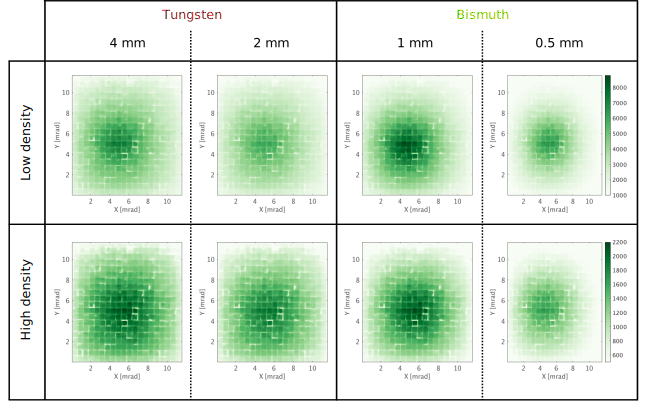
\includegraphics[width=1.\columnwidth]{BW_GammaProfileConverter_Montage.pdf}

\caption[Montage of averaged gamma profile measurements for different materials and accelerator settings.]{Montage of over 10 shots averaged gamma profile images for different materials and accelerator configurations. The rows (vertical) indicate the accelerator configuration the image is representative of, whereas each column refers to a different target material or thickness. The thickness of targets decreases from left to right. The colour scale shows the number of pixel counts on the camera which is proportional to the number of emitted scintillation photons per ${mrad}^2$. The images on the top row and the images on the bottom row are at the same colour scale, respectively.}
\label{BW:figs:Gprofile_materials_montage}
\end{figure}

An overview of the of the targets is shown in Table \ref{BW:tables:brems_converters}.
The materials used in this experiment are tungsten (W) and bismuth (Bi). Both are high-Z materials ($Z = 74$ and $83$), which means energy can be efficiently converted to radiation within thinner targets resulting in less scattering and divergence \cite{Stearns1949_Brems,Jackson}. Tungsten is very dense at $\rho = 19.3\,\mathrm{g/cm^3}$, whereas bismuth is about half as dense \cite{PDG_ATOM}. Both materials are also readily available and easy to handle. The converter materials were mounted on $0.5\,\mathrm{mm}$ plastic (PTFE) and placed on a motorised linear stage that allows switching between the materials or removing the converter targets from the beam path completely. 
The specific target thicknesses used were $2\,\mathrm{mm}$ and $4\,\mathrm{mm}$ for tungsten (W), which correspond to just over $0.5$ and $1$ radiation lengths, $X_0$ \cite{Jackson,PDG_ATOM}. The bismuth (Bi) targets were $0.5$ and $1\,\mathrm{mm}$ thick, which corresponds to $0.08$ and $0.15 X_0$. From the thicknesses and radiation lengths we expect that the tungsten targets will convert more of the electron energy into bremsstrahlung but that the bismuth targets produce a more collimated beam of radiation \cite{Stearns1949_Brems}. We will investigate this in the following. We also consider two accelerator configurations, one using a higher electron density which produces electron beams of higher charge and divergence but lower maximum energy, the other one at lower density which produces higher energies at lower beam charge and divergence. For each target and accelerator setting 10 shots were taken. Figure \ref{BW:figs:Gprofile_materials_montage} shows a montage of the averaged gamma profile response at each configuration.
\vspace{\baselineskip}

\begin{figure}
\centering
\includegraphics[trim={4.9cm 0 5cm 0}, clip, width=.9\columnwidth]{2018QED_Converter_Yield.png}
\caption[Gamma-ray yield of the bremsstrahlung source for tungsten and bismuth at different accelerator settings.]{Total measured gamma yield of the gamma-ray beam at two accelerator configurations (low and high electron densities) for tungsten (W, red) and bismuth (Bi, yellow). The values for the thin and the thick targets are shown by the thin and thick bars, respectively. The error bars indicate the standard deviation from the mean assuming a normal distribution of the data.}
\label{BW:figs:BarConverter_Yield}
\end{figure}


In Figure \ref{BW:figs:BarConverter_Yield}, the average yield of gamma-rays measured on the gamma profile screen for each of the configurations is presented in form of a bar chart, where each bar represents the average of a 10-shot dataset and the error bars indicate the standard deviation. The materials are colour-coded, with results related to tungsten coloured in red and bismuth in yellow. The thick red bars indicate that the thicker tungsten target ($d = 4\,\mathrm{mm}$) was used, the thin bar relates to the thinner target ($d = 2\,\mathrm{mm}$). Similarly, the thick yellow bar corresponds to the bismuth target of thickness $d = 1\,\mathrm{mm}$ and the thin one for $d = 0.5\,\mathrm{mm}$. The bars are presented in two groups, one labelled with `low density', the other one with `high density', which relates to the configuration of the accelerator.

In general, the bremsstrahlung source achieves consistently a higher yield at the `low density' configuration. In all configurations thicker targets produce a higher yield than their thin counterparts of the same material. This trend is more pronounced for bismuth. Despite the different thicknesses the yield is very similar at each configuration, with mainly the thin bismuth target producing a significantly lower yield.
\vspace{\baselineskip}

\begin{figure}
\centering
\includegraphics[trim={4.9cm 0 5cm 0}, clip, width=.9\columnwidth]{2018QED_Converter_Divergence.png}
\caption[Divergence of the gamma-ray beam for tungsten, bismuth and different accelerator settings.]{\textsc{fwhm} divergence of the gamma-ray beam at two accelerator configurations (low and high electron densities) for tungsten (W, red) and bismuth (Bi, yellow). The values for the thin and the thick targets are shown by the thin and thick bars, respectively. The error bars correspond to $\pm1$ standard deviation from the mean under the assumption of a normal distribution.}
\label{BW:figs:BarConverter_Divergence}
\end{figure}

The \textsc{fwhm} divergence of the measured radiation profiles is shown in a similar format in Figure \ref{BW:figs:BarConverter_Divergence}. 
The divergences are in general larger at high densities than at low densities, which might be due to the larger initial divergence of the electron beam, $\theta_e$, and the decrease in energy. We expect the divergence of the radiation to roughly scale as \cite{Stearns1949_Brems}
\begin{equation}
\theta \sim \theta_e + \frac{\ln\gamma}{\gamma},
\end{equation}
where the divergences of the radiation cone and the electron beam are additive.
In all configurations the divergence is $> 6\,\mathrm{mrad}$. At a fixed accelerator configurations, thicker targets result in more divergent radiation, which might be due to small-angle scattering of the electron beam in the material \cite{Moller1932_Moller,Bethe1953_Moliere}. The radiation with the lowest divergence was measured using the thinnest target, bismuth of $d = 0.5\,\mathrm{mm}$, also at the low density configuration of the accelerator. The thin bismuth target, however, produced the lowest yield, which indicates that yield and divergence have to be weighted against each other. The low density configuration seems to be favourable for the accelerator.
\vspace{\baselineskip}

Finally, the pointing variations of the gamma-ray beam are shown in Figure \ref{BW:figs:converter_pointing}. The pointing should not be material-dependent but inherited from the electron beam \cite{Stearns1949_Brems}. In all cases the pointing of the beam centroid is $> 1\,\mathrm{mrad}$, reaching a maximum for the thin tungsten targets at just over $1.7\,\mathrm{mrad}$ at both accelerator configurations. However, there does not seem to be a general trend as for the divergence and the yield, which indicates that these fluctuations are due to variations in the electron beam performance and not due to the change in converter material.
\vspace{\baselineskip}

\begin{figure}
\centering
\includegraphics[trim={4.9cm 0 5cm 0}, clip, width=.9\columnwidth]{2018QED_GConverter_Pointing.png}
\caption[Pointing of the gamma-ray beam for the different materials and accelerator settings.]{Pointing of the gamma-ray beam at two accelerator configurations (low and high electron densities) for tungsten (W, red) and bismuth (Bi, yellow). The values for the thin and the thick targets are shown by the thin and thick bars, respectively.}
\label{BW:figs:converter_pointing}
\end{figure}

The survey of the gamma-ray beam properties so far has shown that thicker targets produce a higher yield of gamma radiation but at cost of increasing the divergence of the beam profile, and that a low density configuration is favourable in either case. The W collimator is $100\,\mathrm{mm}$ long and its aperture permits an optical field of view of $7.14 \pm 0.1 \,\mathrm{mrad}$ full angle, with an acceptance angle at its entrance of $11.11\pm0.1\,\mathrm{mrad}$. The choice of material is then based on the effective yield that is transported through the collimator and is then incident on the interaction point.
An example of a gamma-profile measurement with and without collimator is shown in Figure \ref{BW:figs:Gprofile_collimator_INOUT}. The circular aperture seen on the profile monitor has a \textsc{fwhm} of $6.2$ mrad which corresponds to $10.5$ mrad width to decay to $1/e^2$ of its peak value, assuming a Gaussian distribution. This is larger than the predicted field of view of $7.14\pm0.1$ mrad and matches more the acceptance angle of the collimator at its entrance. The soft edges indicate this is due to hard and slowly expanding radiation penetrating parts of the collimator.
\begin{figure}
\centering
\includegraphics[trim={1cm 0 1cm 0}, clip, width=.5\columnwidth]{BW_GammaProfile_Example.png}\includegraphics[trim={1cm 0 1cm 0}, clip, width=.5\columnwidth]{BW_GammaProfileCollIN_Example.png}

\caption[Gamma profile measurements with collimator in and out.]{Examples of gamma profile measurements of the bremsstrahlung source with the tungsten collimator in (right) and out (left) in units of mrad. The x-axis indicates the divergence in the horizontal direction, the y-axis in the vertical axis. The colour scale indicates the number of pixel counts on the camera which is proportional to the number of emitted scintillation photons per ${mrad}^2$.}
\label{BW:figs:Gprofile_collimator_INOUT}
\end{figure}

Considering the collimator and the measured divergences of the gamma rays, we can now estimate the fraction of the gamma-ray beam that will be transmitted through the collimator.
We will use the measured \textsc{fwhm} divergence values and model the intensity profile after a two-dimensional Gaussian. We will also assume that the peak of the distribution is centred on the collimator and ignore any beam pointing as it does not depend on the material. We then integrate in both dimensions up to a transverse cut-off at $11.11\,\mathrm{mrad}$, assuming that any radiation beyond this angle is terminated efficiently by the collimator. The transmitted gamma yield estimated this way is shown in Figure \ref{BW:fig:abs_transmission}. Similarly as before, the low-density accelerator achieves a higher yield as the high density configuration due to its lower initial yield and higher divergence. In general, thicker targets still transmit a higher yield of gamma rays than their thinner counterparts of the same material. The highest transmitted yield is achieved using bismuth of thickness $d = 1\,\mathrm{mm}$, followed by tungsten of $d = 4\,\mathrm{mm}$. Based on this bismuth of $d = 1\,\mathrm{mm}$ in a low density configuration of the accelerator seems to be the most suitable choice for the bremsstrahlung source as the highest yield is transported to the interaction point.

\begin{figure}
\centering
\includegraphics[trim={4.9cm 0 5cm 0}, clip, width=.9\columnwidth]{2018QED_AbsTransmission_V3.png}
\caption[Estimated through collimator transmitted gamma-ray yield for different materials and accelerator settings.]{Estimated transmitted yield through the collimator assuming a cut-off at 11.11 mrad at two accelerator configurations (low and high electron densities) for tungsten (W, red) and bismuth (Bi, yellow). The values for the thin and the thick targets are shown by the thin and thick bars, respectively. The error bars indicate the standard deviation from the mean value assuming a normal distribution.}
\label{BW:fig:abs_transmission}
\end{figure}

\subsubsection{Background candidate events}

The positrons produced by the Breit-Wheeler process are detected by the TimePix3 detectors\footnote{The detectors were provided by the MediPix Collaboration (CERN) and the data was analysed by Brendan Kettle (Imperial College).}. These are sensitive to gamma rays and charged particles over a wide range of energies. The shape of the tracks in the detector allows some events to be excluded. For example, low energy charged particles produce wiggly tracks, high energy particles or gammas produce straight tracks, the length of which provides information about the angle of incidence. As positrons transported through the magnetic chicane from the collision point enter the detectors within a specific range  of angles, this can be used to exclude some high energy events. Events which are not excluded are `candidate events'.

\begin{figure}
\centering
\includegraphics[trim={4.0cm 0 5cm 0}, clip, width=.9\columnwidth]{2018QED_Converter_YieldvNoise_V3.png}
\caption[Candidate events on the TimePix detectors as function of gamma-ray yield for tungsten (W) and bismuth (Bi).]{Candidate events on the TimePix detectors as function of the yield measured on the gamma profiles for tungsten (W, red) and bismuth (Bi, yellow). The large squares indicate results from thick, the smaller ones from thin converter targets. The gradients indicate a material-dependent noise-to-yield ratio.}
\label{BW:figs:converter_noise_div_yield}
\end{figure}
Gamma rays can interact with material in the chamber (e.g. the magnets, lead walls, Kapton tape) and produce positrons via the Bethe-Heitler process that have similar characteristics (energy, angle into the chicane) so that they are indistinguishable from Breit-Wheeler positrons on the detector. Gamma rays striking the vacuum windows can also scatter into the detector at the angle corresponding to a candidate event.  
We might expect that the number of these noise events will depend on the gamma yield. The following section examines this for the previously discussed scenarios.
\vspace{\baselineskip}

\begin{figure}
\centering
\includegraphics[trim={4.0cm 0 5cm 0}, clip, width=.9\columnwidth]{2018QED_YieldvNoise_CollIN_V3.png}
\caption[Candidate events on the TimePix detectors as function of gamma-ray yield with the collimator in the beam path.]{Candidate events on the TimePix detectors as a function of gamma-ray yield with the collimator in the beam path (cyan). The noise-yield gradients for tungsten (red) and bismuth (yellow) from Figure \ref{BW:figs:converter_noise_div_yield} are indicated as comparison.}
\label{BW:fig:Yield_with_Coll}
\end{figure}
The number of background candidate events measured on the TimePix3 detector is shown in Figure \ref{BW:figs:converter_noise_div_yield} as a function of the gamma yield on the same shot. Here we only considered the results taken at the `low density' configuration of the accelerator, where red markers again indicate results from tungsten targets and yellow from bismuth targets, respectively. Larger markers refer to results from thick and smaller markers to results from thinner targets. For each material the gamma yield seems to correlate well linearly with the number of measured candidate events. The linear correlation coefficient for tungsten is $0.97$ and for bismuth $0.95$. The gradient of the linear fit indicates the number of background candidate events produced per yield measured on the gamma profile detector, i.e. is an indicator of noise over yield (which is used to generate a signal). The inverse of the gradient is then an indicator of yield over noise or signal to noise. The gradient for tungsten is steeper than for bismuth which indicates that more noise is being produced per unit yield reaching the gamma detector. This could be due to stronger scattering of the electron beam in the material which results in more gamma rays being emitted at angles that allow for interaction with the magnet and shielding apertures. Interestingly, the thickness of the targets itself does not seem to have an as large impact on the noise production as the material itself.
\vspace{\baselineskip}

\begin{figure}
\centering
\includegraphics[trim={4.9cm 0 5cm 0}, clip, width=.9\columnwidth]{2018QED_Yield_CollIN_V2.png}
\caption[Total measured gamma yield at low density accelerator configuration for tungsten (W) and bismuth (Bi).]{Total measured gamma yield at low density accelerator configuration for tungsten (W, red) and bismuth (Bi, yellow). In turquoise the gamma yield measured using the thick bismuth target and the collimator in the beam path. The values for the thin and the thick targets are shown by the thin and thick bars, respectively. The error bars are the standard deviation from the mean assuming a normal distribution of the data.}
\label{BW:fig:Yield_with_Coll_bar}
\end{figure}
\begin{figure}
\centering
\includegraphics[trim={4.9cm 0 5cm 0}, clip, width=.9\columnwidth]{2018QED_SignalToNoise_CollIN_V3.png}
\caption[Inverse of fitted gradient (yield over noise) from Figure \ref{BW:fig:Yield_with_Coll} at low density accelerator configuration for tungsten (W) and bismuth (Bi).]{Inverse of fitted gradient (yield over noise) from Figure \ref{BW:fig:Yield_with_Coll} at low density accelerator configuration for tungsten (W, red) and bismuth (Bi, yellow). In turquoise the gradient fitted for the data using the thick bismuth target and the collimator in the beam path.}
\label{BW:fig:Yield_with_NoiseColl_bar}
\end{figure}
Figure \ref{BW:fig:Yield_with_Coll} shows the same relation but this time including a dataset with the tungsten collimator in the beam path (cyan), but also showing the linear fits for tungsten (red) and bismuth (yellow) without the collimator as reference. For this dataset we used the optimum conditions determined so far (low density, bismuth at $d = 1\,\mathrm{mm}$). The gamma yield and the number of candidate events is much lower than the results presented in Figure \ref{BW:figs:converter_noise_div_yield}, but we also see that the gradient of the linear fit relating to the data with the collimator is much lower than for the data without. Figure \ref{BW:fig:Yield_with_Coll_bar} shows a comparison of the total yield with and without the collimator, similar to Figure \ref{BW:figs:BarConverter_Yield} but including the new dataset. We see that introducing the collimator reduced the yield from the related scenario by more than a factor of $10$, which is more than we expected based on the field of view of the collimator. The discrepancy might be due to misalignment of the source and the collimator. In Figure \ref{BW:fig:Yield_with_NoiseColl_bar} the inverse of the gradients of the linear fits are shown for the different scenarios. This value is an indicator for the signal to noise ratio. As already seen in Figure \ref{BW:figs:converter_noise_div_yield} the gradient is steeper for tungsten than for bismuth, almost by a factor 2, such that its inverse is smaller by the same amount. This means that for the same yield of gamma rays twice the amount of background events with similar properties like the Breit-Wheeler pairs we will attempt to measure will be produced and measured at the plane of the single-particle detectors. The inverse of the gradient for the dataset with the collimator is even larger by a factor 7 from bismuth. This clearly shows that the collimator is performing as intended. It does not just reduce the yield but improves the signal-to-noise ratio at the plane of the single-particle detectors by spatially filtering the components of the radiation that are most likely to generate Bethe-Heitler pairs.

\subsubsection{Summary}

In this section, we compared the performance of a LWFA driven bremsstrahlung source for tungsten and bismuth at two thicknesses and two accelerator configurations. We found that the highest yields were achieved at the low-density configuration of the accelerator and thicker converter targets produce higher radiation yields. Tungsten of thickness $d = 4\,\mathrm{mm}$ and bismuth of $d = 1\,\mathrm{mm}$ reached the highest yields. The divergences of the radiation profiles were found to be larger for thicker targets and the high-density configuration of the accelerator, but $> 6\,\mathrm{mrad}$ in all settings. Factoring in the field of view of the tungsten collimator, the effective yield reaching the interaction point was the highest for bismuth of thickness $d = 1\,\mathrm{mm}$. We also considered the correlation of gamma yield and the production of noise in form of background candidate events measured by the TimePix3 detectors that are used to measure the positrons created in the Breit-Wheeler process. A material-dependent linear relation was found linking measured gamma yield and the number of detected candidate events. The number of events generated per gamma yield was lower for bismuth than for tungsten, which again favours bismuth as choice. In this context we also confirmed that the tungsten collimator performs its function well and improves the signal to noise by a factor of 7 relative to the relation found for bismuth. 
As a result, bismuth of thickness $d = 1\,\mathrm{mm}$ at a low density configuration appears to be the best choice as it produces the highest yield reaching the interaction point through the collimator and generates the lowest amount of noise in form of background candidate events.


\section{Characterisation of Gamma Spectra}
\label{BW:sec:GammaCharac}

We determined the optimum conditions for the bremsstrahlung source and characterised the variations in the electron spectra on the three shot days. We will now characterise the gamma spectra for the relevant shot days at the optimum conditions identified before.
Due to the intrinsic variations of the wakefield accelerator characterised in Section \ref{BW:sec:Espec}, we also expect the emitted gamma spectrum to vary on those days. To estimate the range of spectra that can be produced on these days, we selected three different examples of electron spectra measured in the experiment, shown in Figure \ref{BW:fig:GSpec_GEANT} (top left). One spectrum (blue) has a very flat energy distribution from $350$ to just under $700\,\mathrm{MeV}$, with a fall-off reaching up to $800\,\mathrm{MeV}$ electron energy. The next spectrum (green) is sharply peaked at $350\,\mathrm{MeV}$ with a slow roll-off up to $800\,\mathrm{MeV}$. The third spectrum is strongly peaked at $450\,\mathrm{MeV}$ electron energy with a shoulder falling off to lower energies and a sharp cut-off at $500\,\mathrm{MeV}$, and a maximum energy reaching just under $600\,\mathrm{MeV}$. We then simulated the bremsstrahlung spectrum produced by these electron spectra in an interaction with a $1\,\mathrm{mm}$ bismuth foil using GEANT4 \cite{GEANT4}. The resulting bremsstrahlung spectra are also shown in Figure \ref{BW:fig:GSpec_GEANT} (top right), where the gamma-ray spectra are coloured as their corresponding electron spectra. Despite the different spectral shapes of the electron spectra the simulated gamma spectra are close in shape and follow the same exponential fall-off for up to $400\,\mathrm{MeV}$. The maximum energies of the radiation spectra match the maximum energies of the related electron spectra, which introduces the main difference between the spectra. The bremsstrahlung process mitigates the intrinsic fluctuations in spectral shape and energy of the wakefield electron beam efficiently and reduces the fluctuations to its high-energy tail, which contributes only a low number of photons to the overall spectrum. 
\begin{figure}
\centering
\includegraphics[width=.5\columnwidth]{2018QED_ElecSpecs_examples2.png}\includegraphics[width=.5\columnwidth]{2018QED_GammaSpec_simspec2.png} 

\includegraphics[width=.5\columnwidth]{2018QED_GammaSpec_simresp_V2.png}\includegraphics[width=.5\columnwidth]{2018QED_GammaSpec_Average_expsim.png}
\caption[Example electron spectra and corresponding in GEANT simulated gamma spectra along with simulated and experimentally measured detector responses.]{Top left: Examples of electron spectra measured in the experiment and used as simulation input. Top right: Resulting gamma spectrum based on GEANT simulations. Bottom left: Simulated detector responses for the simulated spectra. Bottom right: Example of an experimentally measured raw response (blue) and corresponding simulation (orange).}
\label{BW:fig:GSpec_GEANT}
\end{figure}

Figure \ref{BW:fig:GSpec_GEANT} (bottom left) shows the response of the gamma spectrometer to the respective gamma spectra: the responses for both peaked spectra (orange and green) are visually not distinguishable, whereas the response for the gamma spectrum reaching the highest energies (blue) is shifted slightly towards to higher crystal numbers. The response of the detector is dominated by the spectrum below $400\,\mathrm{MeV}$ and is not able to clearly resolve a spectral change as induced by the variation in spectra shown. An example of an experimentally measured response curve is shown in Figure \ref{BW:fig:GSpec_GEANT} (bottom right). Due to experimental uncertainties of background noise and imperfections in the detector setup, we are also not able to measure the small difference in the responses shown in Figure \ref{BW:fig:GSpec_GEANT} (bottom left) which would have given indication of significant changes in the spectrum. As we are unable to measure the electron beam on-shot when the converter targets are inserted into the beam path, we are not able to resolve any shot-to-shot fluctuations in the high-energy tail of the gamma spectrum on-shot. Instead we are limited to only confirm experimentally that the bremsstrahlung source performs, within the limits of the detector, reliably and consistent with simulations, generating comparable spectra on all three days. The spectrometer also provides the on-shot yield of the radiation which is linearly correlated with the yield measured on the gamma profile screen at a correlation coefficient of $>0.99$, so that either diagnostic provides an equivalent measurement of this observable.
\begin{figure}
\centering
\includegraphics[trim={4.5cm 0 5cm 0}, clip, width = 0.9\columnwidth]{2018QED_GEANT_AvGSpec_V2.png}
\caption[Simulated average gamma spectra for the relevant shot days based on average electron spectra measured in the experiment.]{In GEANT4 simulated average gamma spectra for the relevant shot days (\textsc{a}, \textsc{b} and \textsc{c}) based on average electron spectra measured in the experiment. The average number of photons per shot per MeV is shown as a function of the photon energy. The spectra were scaled relative to each other such that their integrated yield matches the measured relative yield of radiation measured experimentally on the shot days.}
\label{BW:fig:GSpec_AverageSpecVariations}
\end{figure}
\begin{figure}
\centering
\includegraphics[trim={4.5cm 0 5cm 0}, clip, width=.9\columnwidth]{2018QED_GSpec_Variations_V2.png}
\caption[Variations of the gamma yield for the relevant shot days.]{Left: Average gamma-ray yield measured with the gamma profile and spectrometer on the shot days \textsc{a} (blue), \textsc{b} (purple) and \textsc{c} (green), normalised to the maximum value in the group. The error bars indicate the standard deviation from the average assuming a normal distribution. Right: Fraction of photons above 400 MeV contributing to the overall spectrum based on the average gamma spectrum for the shot days as simulated in GEANT4 using the average electron spectra. The error bars indicate the change induced by the standard deviation on the spectral shape of the average electron beam.}
\label{BW:fig:GSpec_Variations}
\end{figure}

In order to nonetheless quantify the variation in performance for the shot days we will rely on the characterisation of the electron beams presented in Section \ref{BW:sec:Espec}. Using the average electron spectrum for each shot day, the corresponding average gamma spectrum can be simulated in GEANT4. As the average electron spectra are representative of the performance of the accelerator on that day, the simulated gamma spectra will also, within limits, reflect the performance of the bremsstrahlung source. It should, however, be noted that this does not capture changes in performance throughout the process of data taking and that this link becomes less reliable the more the characterisation of the electron source and a particular data shot are separated in time. However, the response measured by the gamma spectrometer in the experiment did not measurably change shape over the course of the days which suggests spectral stability within the sensitivity of the detector arrangement. The average gamma spectra for the shot days, simulated in GEANT4 using the average electron spectra, are shown in Figure \ref{BW:fig:GSpec_AverageSpecVariations}. The spectra were scaled relative to each other to reflect the proportionality of the experimentally measured yield of gamma-rays on the respective shot days. The simulated gamma spectra for days \textsc{b} (purple) and \textsc{c} (green) are similar in spectral shape with a cut-off at a photon energy of just under $700\,\mathrm{MeV}$ and $600\,\mathrm{MeV}$, respectively. The electron spectra reached on average higher maximum energies on day \textsc{a} (blue) which results in also producing the highest energy photons with a cut-off in the gamma spectrum at a photon energy of $800\,\mathrm{MeV}$. The total radiation yield for the shot days is shown in a bar chart in Figure \ref{BW:fig:GSpec_Variations}. The group on the left shows the average radiation yield that was measured experimentally on that day. The error bar indicates the standard deviation in the data set and the height of the bars were normalised to the maximum value in the group. The measured radiation yield was the highest on day \textsc{a} (blue), followed by day \textsc{b} (purple) and day \textsc{c} (green), each spaced by about $20\%$. The group on the right shows the proportion of photons above $400\,\mathrm{MeV}$ within the entire spectrum on the respective days, now considering the simulated average gamma spectra shown in Figure \ref{BW:fig:GSpec_AverageSpecVariations}. The values are normalised by the maximum value in the group. The error bars reflect the changes in the spectrum due to the standard deviation of the electron spectrum. The group was also normalised to the maximum value in the group. As already indicated in Figure \ref{BW:fig:GSpec_AverageSpecVariations} the number of photons above $400\,\mathrm{MeV}$ was the highest in relative and absolute terms on day \textsc{a} (blue), followed by day \textsc{b} (purple) and then day \textsc{c} (green).
In short, the bremsstrahlung source performed the best in terms of yield on day \textsc{a}, followed \textsc{b} and \textsc{c}, and also emitted higher energy radiation on day \textsc{a}, based on the performance of the electron source characterised in Section \ref{BW:sec:Espec}.



\section{Characterisation of X-ray spectra}
\label{BW:sec:Xrays}

\begin{figure}
\centering
\includegraphics[trim={4cm 0 5cm 0}, clip, width=.9\columnwidth]{BW_XraySpec_Morton_V2.png}

\includegraphics[trim={4cm 0 5cm 0}, clip, width=.9\columnwidth]{BW_XraySpec_AvDay_V3.png}
\caption[X-ray spectra produced with the burn-through foil. Simulated and experimentally measured X-ray spectra.]{X-ray spectra produced with the burn-through foil. Top: Simulated X-ray spectra for a 5 keV energy window as emitted by 100 nm germanium target heated by a high-intensity laser pulse. The y-axis indicates the number of photons per keV, the x-axis the energy of the X-ray photons (blue) and after being filtered by $5\,\mathrm{\upmu m}$ of Kapton as used in the experiment (red). The dashed yellow lines indicate the spectral interval measured with the crystal spectrometer in the experiment. Bottom: X-ray spectra measured experimentally averaged for each of the three shot days \textsc{a}, \textsc{b} and \textsc{c} using a crystal spectrometer setup. The shaded regions indicate the standard deviation from the mean assuming a normal distribution.}
\label{BW:Figs:Xray_Sim_and_Exp}
\end{figure}

The X-rays are generated by a laser beam of pulse duration $40$ ps \textsc{fwhm} heating a burn-through foil \cite{Edwards1990_BURNTHROUGH} and are emitted approximately in a $4\pi$ solid angle. The target is a thin $100\,\mathrm{nm}$ coating of germanium on a $5\,\mathrm{\upmu m}$-thick Kapton tape as base. The X-rays travelling to the interaction point traverse the plastic tape which results in a filtering of low energy X-rays. 
In the experiment, the X-ray source is characterised by a pinhole camera and a crystal spectrometer. The pinhole camera measures the source size and flux, and the crystal spectrometer measures the X-ray spectrum. Both diagnostics measure the X-rays from the side the foil is heated from, which means it is not filtered by the Kapton tape. The analysis of the X-ray data has been conducted by Cary Colgan (Imperial College) and Brendan Kettle (Imperial College). John Morton (AWE) provided simulations of the emitted X-ray spectra. Based on the X-ray yield the preliminary estimate for the conversion efficiency from laser light into X-rays between $1.3$ to $1.9\,\mathrm{keV}$ was about $4.9\pm0.3$ percent.
\vspace{\baselineskip}

The simulated X-ray spectrum is shown in Figure \ref{BW:Figs:Xray_Sim_and_Exp} (top) with filtering (red) and without filtering (blue) by the Kapton tape.
The spectrum exhibits two distinct emission peaks, one between $1.2$ and $1.5\,\mathrm{keV}$, another lower one between $1.6$ and $1.9\,\mathrm{keV}$. The spectrum underlying these two emission peaks appears to fall off exponentially from lower to higher X-ray energies, such that the emission peaks are $2-3$ orders of magnitude higher than the surrounding spectrum. When including the spectral filtering of the radiation by the layer of Kapton, most of the photons below $1\,\mathrm{keV}$ X-ray energy are cut out efficiently with exception of the spectral K-edge which leaves a narrow bandwidth at photon numbers comparable to the high emission peak. The experimentally measured spectral range is marked in the simulation data presented in Figure \ref{BW:Figs:Xray_Sim_and_Exp} (top) with two yellow dashed lines.
\vspace{\baselineskip}
\begin{figure}
\centering
\includegraphics[trim={4.9cm 0 5cm 0}, clip, width=.9\columnwidth]{BW_Pinhole_Pinhole_Yield_V4.png}

\includegraphics[trim={4.9cm 0 5cm 0}, clip, width=.9\columnwidth]{BW_CSpec_Pinhole_Yield_V4.png}
\caption[X-ray yield measured with the pinhole camera and the crystal spectrometer. ]{X-ray yield measured with the pinhole camera and the crystal spectrometer. Top: Comparison of the yield measured through both pinholes. The yield on pinhole 2 (filtered with mylar) as a function of the yield on pinhole 1 (filtered with aluminium). Bottom: The yield detected with the pinhole camera, separately for the two pinholes, one filtered with aluminium (red) and the other one with mylar (yellow), as a function of the yield measured with the crystal spectrometer.}
\label{BW:Figs:Xray_Pinhole_CSpec_Yield}
\end{figure}

Similarly as before, we will characterise the properties of the source on the three shot days \textsc{a}, \textsc{b} and \textsc{c}. The average spectra measured by the crystal spectrometer on the three days are shown on a logarithmic $y$-scale in Figure \ref{BW:Figs:Xray_Sim_and_Exp} (bottom), with the standard deviation of the shot-to-shot fluctuations from the mean indicated in the shaded regions. The range of X-ray energies shown on the $x$-axis is representative of the spectral range measured effectively with the crystal spectrometer setup throughout the three shot days. The measured spectrum falls off sharply on either side of the spectral window presented here as the end of the crystal is reached. The height of the spectra is indicative of the relative X-ray yield on the different days. The distinct peaks are emission lines of the material and slight spectral shifts are due to smaller calibration and alignment errors. 
The spectral shape on day \textsc{b} and \textsc{c} is very consistent, whereas on day \textsc{a} the spectral lines above $1.4\,\mathrm{keV}$ are less pronounced and the spectrum falls off. This is probably due to varying plasma conditions as a hotter or colder plasma will shift the emission lines and rates. The spectrum on day \textsc{a} is also cut off at around $1.33\,\mathrm{keV}$, which is due to misalignment of the crystal and not a physical phenomenon. In general, the shape of the X-ray spectra is consistent from shot-to-shot, whereas the shaded regions indicate that the total yield of photons can change significantly.
\vspace{\baselineskip}
\begin{figure}
\centering
\includegraphics[trim={4.9cm 0 5cm 0}, clip, width=.9\columnwidth]{BW_XraySpec_AvDay_Yield_V3.png}
\caption[Average X-ray yield as measured by the crystal spectrometer on the different shot days.]{Average X-ray yield as measured by the crystal spectrometer on the different shot days (\textsc{a},\textsc{b} and \textsc{c}) normalised by the maximum X-ray yield in the group. The error bars indicate the standard deviation of the total yield for the respective shot day assuming a normal distribution.}
\label{BW:Figs:Xray_Yield}
\end{figure}

The yield of the X-ray source is measured by a pinhole camera setup with two pinholes, one filtered with aluminium, the other one with PTFE. The X-ray yield for an example dataset is shown in Figure \ref{BW:Figs:Xray_Pinhole_CSpec_Yield}. On the top, the yield measured through both pinholes is compared. The measured quantities are linearly correlated at a correlation coefficient of $0.99$, which indicates that the relative distribution of photons in the spectrum, i.e. the spectral shape, remains consistent throughout the shots or that changes only occur in a spectral region that causes the same response for both pinholes (above $1\,\mathrm{keV}$ \cite{HENKE}).
On the bottom, the yield measured by the crystal spectrometer in the limited spectral window is shown together with the yield measured by the pinhole camera setup on the same shots. Both pinhole measurements correlate linearly with the result from the crystal spectrometer at a correlation coefficient of $0.90$. This indicates that the spectral range measured by the crystal spectrometer contributes consistently a similar fraction to the overall yield as measured through either pinhole camera, which in turn confirms the consistency of the spectral shape on a shot-to-shot basis.
As a result, the yield measured by the crystal spectrometer is also a good indicator for the relative changes in the yield of the entire X-ray emission. Overall we can observe that shot-to-shot yield varies significantly, but there are strong indications that the spectral shape remains consistent. 

Returning to the variations in performance of the X-ray source, the average X-ray yield on the three shot days is shown relative units in a bar chart
in Figure \ref{BW:Figs:Xray_Yield}, where the error bars indicate the standard deviation from the mean. The average yield is very consistent on days \textsc{b} and \textsc{c}, but was about $30\%$ lower on day \textsc{a}. However, on all three days the standard deviation is large at $>30\%$ of the mean value, reaching $>50\%$ on day \textsc{a}. Determining the absolute X-ray yield and its temporal distribution are still subject of the ongoing analysis.


\section{Spatio-temporal overlap of photon sources}
\label{Chap:BW:Sec:Overlap}

\begin{figure}
\centering
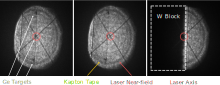
\includegraphics[width=.9\columnwidth]{BWXrayAlignment.png}
\caption[Alignment of the germanium (Ge) X-ray target relative to the wakefield beam axis.]{Alignment of the germanium (Ge) X-ray target relative to the wakefield beam axis (red circle). The cross-hair indicates the centre of the wakefield driver beam. First, the Ge target is placed on the beam axis (left). Then it is translated 1 mm away from the axis (centre) and the side of the driver beam containing the X-ray target is blocked by an tungsten (W) block.}
\label{Chap:BW:Figs:GeTargetAlignment}
\end{figure}


In order to produce electron-positron pairs from the Breit-Wheeler process we have to overlap the high-energy photons emitted from the two sources in time and space.
The two laser pulses driving the photon sources were spatially overlapped to within the width of a thin metal alignment wire $\sim 100\microns$. They were then synchronised to each other to within an accuracy of $\pm 3\picos$ using a fast photodiode and a suitable oscilloscope (see Section \ref{Methods:Sec:DiodeTiming}). The wakefield driver beam is $45\pm5\fs$ long and the pulse duration of the X-ray heater beam is $40\picos$ \textsc{fwhm}.

The typical temporal shot-to-shot fluctuations between the two laser arms at \textsc{Gemini} were measured to be of order of $10's \fs$ with slow long-term drifts of up to $\sim 100\fs$ in more extreme cases (see \cite{Shalloo_GEMINIDRIFT} and Section \ref{Methods:Sec:TimingStability}). Considering the long pulse duration of the X-ray heater beam these fluctuations are negligible.
The LWFA electron bunch that produces the gamma ray beam is delayed relative to the laser driver (see Section \ref{Methods:Sec:Beam_Laser_Timing}). For a gas target of length $17.5\mm$ and density $\sim 2\times 10^{18}\,\mathrm{cm^{-3}}$ this is at most $\sim 180\fs$, which by itself is also negligible. The heated X-ray target, on the other hand, is expected to almost instantaneously produce X-rays. Combining all components discussed so far the centres of the laser pulses are at most temporally offset by $< 3.5\picos$ such that the temporal overlap is guaranteed throughout. Shot-to-shot fluctuations are in general expected to be negligible.
\vspace{\baselineskip}

After having considered the temporal overlap we will now discuss the spatial overlap. The gamma ray beam that is transmitted through the collimator is confined to a cone of $10.5\mrad$ divergence (see Section \ref{BW:sec:GammaCommission}), which expands to a beam size of $(9.01 \pm 0.05) \mm$ at the interaction point located $865 \pm 4.5 \mm$ downstream from the converter target. A tungsten block is used to bisect the gamma ray beam to shield the X-ray target tape from direct gamma hits such that the beam size is halved to $(4.54\pm 0.03) \mm$ (see Figures \ref{Chap:BW:Figs:GeTargetAlignment} and \ref{Chap:BW:Figs:OverlapSpatialTemporal}). The shot-to-shot pointing fluctuations of the gamma ray beam were measured to be $1.2\mrad$ which corresponds to a spatial shift of $1.04\mm$ at the interaction point. However, we expect any pointing variations to be mitigated by the tungsten block and the collimator such that spatial shifts simply result in different parts of the beam being transmitted.

\begin{figure}
\centering
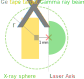
\includegraphics[width=.3\columnwidth]{BWOverlapSketchFront.png}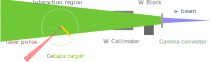
\includegraphics[width=.7\columnwidth]{BWOverlapSketch.png}
\caption[Sketch of the spatial overlap between the two high-energy photon sources.]{Sketch of the spatial overlap between the two high-energy photon sources. Right: Sketch of the top-down view of the interaction region. The electron beam (blue, on the right) passes through a gamma converter (brown) producing gamma radiation (green) from bremsstrahlung. Half of the beam is blocked by a thick tungsten (W) block and the remaining radiation is spatially filtered in a long W collimator. The remaining collimated half circle of radiation is then incident on the interaction region. The X-ray source is driven by a laser pulse that heats a germanium dot (grey) on a Kapton tape (yellow). The X-rays are emitted in $4\pi$ such that a sphere of X-rays is formed around the heated target (dashed circle), with an expanding radius $r_X$. The intersection of the sphere and the half-circle is the interaction region. Left: Sketch of the front view showing the position of the germanium target relative of the laser axis (red cross) and the overlap region of the X-ray sphere (dashed circle) and the transmitted gamma ray beam (green half-circle).}
\label{Chap:BW:Figs:OverlapSpatialTemporal}
\end{figure}
The X-rays, on the other hand, are emitted from $1\pm0.1\mm$ off-axis in a $4\pi$ sphere that expands over time. At the arrival of the gamma ray beam the radius is $> 5.95\mm$, such that the region beyond the laser axis is at least $4.95\pm0.1\mm$ wide. The half-sphere of X-rays crossing the laser axis and the half circle of gamma rays are of comparable size, and it is expected that both fully overlap with each other even in the previously identified largest timing offset of $3.5\picos$ (see Figure \ref{Chap:BW:Figs:OverlapSpatialTemporal}). As a result, we can safely assume that both photon sources will consistently overlap in space and time. If we assume that the temporal intensity profile of the X-ray heater is related to the temporal X-ray yield, a temporal offset of the relative beam timing results in a systematic shift in the number of X-rays that share an interaction volume with the gamma ray flash, where a late arrival of the X-ray heater increases this number.


\section{Variations in the number of produced pairs}

In the previous sections, we characterised the experimental fluctuations of the two photon sources for the three shot days \textsc{a}, \textsc{b} and \textsc{c}.
We showed that due to fluctuations in the electron beam the performance of the bremsstrahlung source also varies from day to day. However, due to the characteristic emission spectrum of the bremsstrahlung process the fluctuations are mainly in the high energy tail of the spectrum and at low photon numbers. These high-energy gamma-rays might still be able to contribute significantly to the total number of pairs produced if their higher energy enables them to interact with a large number of low-energy photons that were not accessible on the shot days \textsc{b} and \textsc{c}. On the other hand, we showed that the performance of the X-ray source was similar for days \textsc{b} and \textsc{c}, but had an about $30\%$ lower average yield of photons on day \textsc{c}. The X-ray yield varied strongly from shot-to-shot at a standard deviation $\sigma >30\%$ of the mean, but the spectral shape remained very consistent on a shot-to-shot basis.
\begin{figure}
\centering
\includegraphics[width=.9\columnwidth]{BWD_Xsec.png}

\includegraphics[width=.9\columnwidth]{BW_Xsec_EgEx_2D_V2.png}
\caption[Breit-Wheeler cross section for a range of X-ray and gamma-ray energies.]{Top: Total Breit-Wheeler cross section, $\sigma_{BW}$, in units of $m^{-2}$ as a function of the centre-of-mass energy, $\sqrt{s}$. Bottom: Total Breit-Wheeler cross section in $m^{-2}$ (colour scale) for an X-ray photon of energy $\epsilon_X$ (y-axis) interacting with a gamma-ray of energy $\epsilon_\gamma$ (x-axis) at an interaction angle of $\theta = 140^\circ$.}
\label{BW:Figs:Xsec_2DRange}
\end{figure}
To estimate the impact of the fluctuations in both photon sources on the number of pairs produced we have to combine both spectral measurements and calculate the Breit-Wheeler cross section, $\sigma_{BW}$, for these interactions.
The Breit-Wheeler cross section depends on the invariant mass of the collision, $s$, which incorporates the energy of the two photons involved in the interaction, $\epsilon_1$ and $\epsilon_2$ and the angle $\theta$ between them:
\begin{equation}
s = \frac{\epsilon_1 \epsilon_2 (1-\cos \theta)}{2 m^2_e c^4}.
\end{equation}

The central angle between the two photon sources was in the experiment set to be $140^\circ \pm 10^\circ$. Due to the strong collimation of the gamma-ray beam to $< 10\,\mathrm{mrad}$ and pointing fluctuations of $< 2\mrad$ the maximum spread of angles is $\theta < 0.7^\circ$ and hence negligible. In this setting the main angular spread is then dominated by the angular distribution of the $\sim 4\pi$ X-ray emission. Due to the wide emission angle of the X-ray source the geometry is less sensitive to angular and spatial variations on a shot-to-shot basis or between shot days, for instance when the tape target is being replaced. Considering this factor and since the analysis of the directionality of the X-ray source is still ongoing, we will for now also ignore any angular variation within the spectrum and calculate the cross-sections at a fixed crossing angle, $\theta$, and investigate how the cross-section, $\sigma_{BW}$, varies for a deviation in $\theta$. 
In Figure \ref{BW:Figs:Xsec_2DRange} (top) the cross section, $\sigma_{BW}$, is shown as a function of the invariant mass, $s$: $\sigma_{BW}$ is zero for $s<1$, then increases up to a peak value at $s = 2$ after which it decays slowly. Since $s \sim \epsilon_1 \epsilon_2$ or in this scenario $s \sim \epsilon_X \epsilon_\gamma$, the energy of the most likely interaction partner for one photon to produce a Breit-Wheeler pair with changes with its energy. For instance, the higher the gamma-ray energy, $\epsilon_\gamma$, the lower the X-ray energy, $E_X$, of the partner photon that would be most likely to produce a pair in an interaction.
In Figure \ref{BW:Figs:Xsec_2DRange} (bottom), $\sigma_{BW}$ is shown for $\theta = 140^\circ$ and a range of X-ray and gamma-ray energies accessible in this experiment. The bulk of the gamma radiation produced in the experiment was in a spectral range up to 400 MeV, which is well matched with the emission peak measured in the X-ray spectrum. The fluctuations of the gamma spectrum in the high-energy tail around 600-800 MeV on the other hand are most likely to interact with X-rays of energy $< 0.4\,\mathrm{keV}$. However, we have seen that this part of the X-ray spectrum is efficiently filtered out by the Kapton base of the burn-through foil, such that the impact of the high-energy fluctuations in the gamma-ray spectrum onto the total cross-section is suppressed.

\begin{figure}
\centering
\includegraphics[trim={4.9cm 0 5cm 0}, clip, width=0.75\columnwidth]{BWXsec_Angles_MortonRawYieldCorr_V2.png}

\includegraphics[trim={4.9cm 0 5cm 0}, clip, width=0.75\columnwidth]{BWXsec_Angles_MortonCorrYieldCorr_V2.png}

\includegraphics[trim={4.9cm 0 5cm 0}, clip, width=0.75\columnwidth]{BWXsec_Angles_AvDay_V2.png}
\caption[Estimated relative number of pairs produced for the three shot days assuming different angles and X-ray spectra.]{Estimated relative number of pairs produced calculated with Equation \eqref{BW:Eqns:NBW} for the three shot days \textsc{a}, \textsc{b} and \textsc{c} at the interaction angles $\theta = 140^\circ \pm 20^\circ$ using the experimentally measured gamma-ray spectrum and a simulated X-ray spectrum (top), a simulated X-ray spectrum including plastic filtering (centre) and using the experimentally measured X-ray spectrum. The error bars indicate the standard deviation from the mean value combining the fluctuations in the X-ray and gamma-ray source, assuming a normal distribution in either case.}
\label{BW:Figs:XsecBarChart}
\end{figure}

We now estimate the average number of pairs produced evaluated for a specific day, $N_{BW,day}$, and at a fixed angle, $\theta$, by combining the spectra of the X-ray source, $\mathrm{d}N_X/\mathrm{d}\epsilon_X$, the gamma-ray spectra, $\mathrm{d}N_\gamma/\mathrm{d}\epsilon_\gamma$, and convolving it with the cross section, $\sigma_{BW}$:

\begin{equation}
\boxed{N_{BW}|_{day,\theta} \sim \int \frac{N_{ph, X}}{\mathrm{d}\epsilon_{X}} \frac{N_{ph, \gamma}}{\mathrm{d}\epsilon_{\gamma}} \sigma_{BW} (\epsilon_{X}, \epsilon_{\gamma}, \theta) \mathrm{d}\epsilon_{\gamma}\mathrm{d}\epsilon_{X}.}
\label{BW:Eqns:NBW}
\end{equation}

We calculate this for the average X-ray and gamma-ray spectra as experimentally measured on the three shot days, but also consider the simulated X-ray spectra presented in Figure \ref{BW:Figs:Xray_Sim_and_Exp} to understand how much the filtering of the X-ray spectrum by the Kapton base affects the result. 
In addition, we consider not only the central angle $\theta = 140^\circ$ but also deviations of $\pm 20^\circ$ to estimate how a global angle would change the number of pairs produced in total but also how much deviation a spread of angles would cause. In the experiment a change in the central angle could, for instance, occur when the spool of tape for the burn-through foil was replaced, or intermittently if the tape was not brought to full tension during the alignment procedure. 
Due to the $4\pi$ emission of the X-ray source, however, this effect is mitigated and a large spread of angles is expected on every shot.
In all cases, we assume that as a prerequisite the gamma-ray beam and the X-rays are overlapped in space and time (see Section \ref{Chap:BW:Sec:Overlap}).
The different values of $N_{BW}$ that were calculated for the different scenarios are presented in the bar chart in Figure \ref{BW:Figs:XsecBarChart}. Since the absolute yield of the photon sources is still subject of an ongoing analysis, here the \textit{relative} variations in $N_{BW}$ between the days and scenarios are considered. The results using the simulated X-ray spectrum, scaled by the experimentally measured X-ray yield, are shown without spectral filtering in the top chart and with filtering in the chart in the centre of the Figure. The chart on the bottom shows the results using the experimentally measured X-ray spectrum. For each chart the relative number of pairs is calculated for three groups using $\theta = 140^\circ\pm20^\circ$ as interaction angle, with the height of the bars normalised to the maximum value of $N_{BW}$ within a chart. The error bars indicate the standard deviation from the average value on a shot-to-shot basis, which is dominated by the variation in the X-ray yield.

For the case of the simulated spectrum without the plastic filter (top) the number of pairs produced for day \textsc{a} is on average the largest, followed by \textsc{b} and then \textsc{c}. This means that the higher gamma-ray yield and peak energy is outweighing the lower X-ray yield.
When including the spectral filtering of the simulated X-rays (centre) the average values for days \textsc{a} and \textsc{b} become more similar. This indicates that the excess of pairs produced on average in the previous scenario are due to low-energy X-rays being able to interact with the high-energy tail of the gamma spectrum measured for day \textsc{a}. By removing the low-energy X-rays from the interaction days \textsc{a} and \textsc{b} equalise as the higher gamma-ray yield on day \textsc{a} is balanced by the higher X-ray yield of day \textsc{b}. The number of pairs is the lowest for day \textsc{c} which has an X-ray yield comparable to day \textsc{b} but a lower gamma-ray yield. 
Using the experimentally measured X-ray spectrum to calculate $N_{BW}$ yields similar results to the simulated X-ray spectra with the plastic filtering, which indicates that the emission line in the X-ray spectrum around $1.5\,\mathrm{keV}$ provides the most important and dominant contribution to the total production of pairs. However, we see that across all three scenarios the highest potential value of $N_{BW}$ on a single shot, not on average, is always expected to be measured on day \textsc{a}, followed by \textsc{b} and then \textsc{c}, due to the large variation in X-ray yield.
Also consistent for all three scenarios is that decreasing the interaction angle, $\theta$, reduces $N_{BW}$.

The changes in the relative number of $N_{BW}$ for the different X-ray spectra shows that we are able to mitigate the influence of the gamma-ray fluctuations by limiting which part of the X-ray spectrum is incident on the interaction point. This is important since we showed that we are not able to resolve the differences in the gamma-ray spectrum on a shot-to-shot basis, resulting in an uncertainty on the expected $N_{BW}$ on each shot. On the other hand, despite the large shot-to-shot fluctuations, the on-shot uncertainty introduced by the X-ray source is small as long as the X-ray yield is measured on-shot.
As a result, within the assumptions made, despite significant variations in the performance of the X-ray and gamma-ray sources, our ability to determine the number of expected pairs on a single shot is not significantly impaired by the limitations in the spectral measurements.
A more detailed analysis including the angular distribution of the X-ray source could, however, alter this conclusion.

\section{Status of the Breit-Wheeler Analysis}

This section aims to place the results presented so far in the context of the overall analysis of the experimental data taken on this campaign and briefly summarise the current status of this analysis, to which a large number of researchers contributed to. Brendan Kettle (Imperial College) had the role as experimental lead, also called `Target Area Operator', during the campaign at \textsc{Gemini} and afterwards coordinated the analysis efforts.
\vspace{\baselineskip}

In order to generate and measure electron-positron pairs from the Breit-Wheeler process, we require two suitable photon sources and a detector system. An overview of the experimental setup aimed at performing this measurement was introduced in Section \ref{BW:sec:expSetup}, at the beginning of this Chapter. The commissioning of the first photon source, a gamma-ray source with hundreds of MeV photon energy, was outlined in Section \ref{BW:sec:GammaCommission}, followed by a characterisation of its performance over the course of three shot days in Section \ref{BW:sec:GammaCharac}. The characterisation of the gamma-ray source and the electron beam that underlies it (see Section \ref{BW:sec:Espec}) consists the main contribution of the author to the overall analysis effort. Section \ref{BW:sec:Xrays} then outlined the properties of the second photon source, an X-ray source and, similarly as for the gamma-ray source, its variations in performance was discussed. The results presented there were contributed by Cary Colgan (Imperial College) and Brendan Kettle (Imperial College), with simulations provided by John Morton (AWE). With both high-energy photon sources commissioned and their performance analysed, the installation of the last component, the detector system for the Breit-Wheeler pairs, has not been discussed in detail yet. This will be corrected in the following.

\subsubsection{Magnetic Chicane}

Since only a small number of pairs is expected to be created in this setup, a magnetic chicane is used to extract only particles with matching properties from the interaction point and guides them onto well-shielded detectors that are capable of detecting single particles. The design, supervision of the positioning and the analysis related to the magnetic chicane were conducted by Dominik Hollatz (Jena). Guillermo Marrero Samarin (QUB) provided FLUKA \cite{FLUKA} simulations to model the generation of background noise and designed the radiation shielding for this setup.

The magnetic chicane consisted of three magnets, one dipole magnet separating the electrons and positrons near the interaction point, and one dipole magnet each on opposite arms to bend the electrons and positrons, respectively, back onto detectors. The magnets for the chicane were set up symmetrically on both sides using identical magnets. The performance of the chicane of tested by removing the dipole magnet that was used as electron spectrometer from the beam path and allowing the electron beam from LWFA to propagate through the electron arm of the chicane. A Lanex screen was inserted after each of the two dipole magnets of the electron chicane. The first screen acted as electron spectrometer, the second screen measured the properties of the electron beam at the end of the chicane equivalent to the measurement plane of the single-particle detectors on the positron arm. The experimental results were consistent with tracking simulations and this result was assumed to hold similarly for the positron arm of the chicane within experimental measurement errors.

\subsubsection{Single-particle detectors}

Two types of single-particle detectors were placed at the end of the positron arm of the magnetic chicane. First, two subsequent silicon-based Timepix3 detectors in order to discriminate particles from noise by tracking lepton hits through both layers. The detectors were provided by the MediPix Collaboration (CERN) and the data was analysed by Brendan Kettle (Imperial College). Second, a caesium-iodide stack coupled to a gated intensified CCD camera capable of identifying single lepton hits. This data was analysed by Guillermo Marrero Samarin (QUB).
Only the positrons were measured as the Breit-Wheeler cross section peaks at $s=2$ resulting together with the asymmetry of the photon energies in an unequal momentum distribution which makes a coincidence measurement more difficult and not feasible in this setup (see Figure \ref{Theory:Figs:BW_DiffXsec_CM_E_LAB_BOTTOM} in Section \ref{Theory:Subsec:BW}).
The single-particle detectors were calibrated by producing Bethe-Heitler pairs with similar properties as the Breit-Wheeler pairs by scattering the gamma-ray beam from solid targets placed on purpose near the interaction point or the gamma-ray axis.
A small cube of tungsten was used to produce a localised source of pairs, whereas a wide scattering screen was re-purposed as wide-angle converter target to produce hundreds of pairs with a momentum distribution that is accepted by the magnetic chicane. With an abundance of signal enough data was produced to identify the characteristic shape and energy deposition of the positrons on both detector types. After removing the calibration sources again the varying background of positrons from the Bethe-Heitler process was characterised on single-beam shots driving either the gamma-ray beam or the X-ray source.

\subsubsection{Photon-photon collider}

Finally, the two photon sources and the single-particle detectors were used simultaneously in dual-beam shots aimed for photon-photon collisions to produce pairs from the Breit-Wheeler process. This was achieved on three shot days at the end of the experimental campaign which in total lasted 8 weeks. The number of weeks required to prepare the experimental setup and to develop the right techniques to reach the stage to take dual-beam shots is indicative of the challenging nature of this experiment. Over the course of the three shot days, for which the variations in the performance of the X-ray and gamma-ray source were characterised in the previous sections, $217$ dual-beam shots were taken for photon-photon collisions and $334$ single-beam shots as background references. The reference and data shots were then used to perform a statistical analysis of the number of registered candidate events to identify whether there was a statistically significant excess of events measured on dual-beam shots, indicating pair production from the Breit-Wheeler process. This analysis was conducted by Brendan Kettle (Imperial College), Guillermo Marrero Samarin (QUB) and Peter Hatfield (Oxford).

\subsubsection{Summary}

In summary, the three components required to produce and measure electron-positron pairs from the Breit-Wheeler process were successfully commissioned and their performance characterised. On three shot days the three components were used simultaneously taking $\sim 200$ dual-beam and $\sim 300$ single-beam reference shots. There was a difference in the number of positrons measured on the dual-beam and single-beam shots indicating potential evidence of pair production from the Breit-Wheeler process. However, this is only a preliminary result and the analysis is still ongoing.


\section{Improvements for a future measurement}
\iffalse
This analysis can be generalised into a design approach considering future measurements of the linear Breit-Wheeler mechanisms at \textsc{Gemini}, summarised by the three methods `stabilise, measure, mitigate'.
\fi

In this section we will discuss, based on the analysis presented in this Chapter, how a potential future measurement of the linear Breit-Wheeler process could be improved. For this discussion we will remain within the framework of the present experimental layout as we were able to field the three main components (gamma-ray source, X-ray source and single-particle detectors) successfully, and we demonstrated that the components worked individually and in tandem as designed. We will in the following discuss how to improve their performance, focusing on the topics of this Chapter, which was mainly the commission of the bremsstrahlung source but also in smaller parts its interplay with the X-ray source.

The bremsstrahlung source in general showed to be producing a directed high-energy gamma-ray beam. The bremsstrahlung process efficiently mitigated the intrinsic spectral variability of the electron beam. Areas of improvement concern the overall yield, spectral shaping, noise production and the resolution of the spectral measurement.
The X-ray source showed to be spectrally very stable, but its yield of X-rays varied strongly from shot to shot. The areas of improvement are hence increasing the stability of the source, further spectral shaping and improving its characterisation.
Finally, the single-particle detectors and the chicane performed as designed, but we will not discuss any alterations to these components here and focus on the light sources instead.

\subsection{Gamma-ray source}

\subsubsection{Laser wakefield accelerator}

In this experiment the electron beam reached a maximum electron energy of $709\pm46\,\mathrm{MeV}$ at an average beam charge of $26.26 \pm 3.8\,\mathrm{pC}$ on the best shot day (\textsc{a}), using $5.51\pm 0.64\,\mathrm{J}$ energy on-target. The laser energy was limited by the damage threshold of the optics in the focusing beam which might have also limited the performance of the accelerator. Electron energies at \textsc{Gemini}, on the other hand, are routinely in excess of $1\,\mathrm{GeV}$ at hundreds of $\mathrm{pC}$ charge \cite{Kneip2009_GEV,Kettle2019_XANES,Hussein2019_MICROSTRUCTURES}, and have in individual cases reached more than $2\,\mathrm{GeV}$ with beam charges of $>300\,\mathrm{pC}$ \cite{Poder2018_RR,PoderThesis}. This indicates that the accelerator was not performing at its optimum and significant improvements of the performance should be possible within the scope of this setup and this laser system. At a fixed electron spectrum, a tenfold increase in beam charge would equally increase the yield of gamma-rays and, as a result, also the number of potentially produced pairs, but also the number of candidate events from noise (see Section \ref{BW:sec:GammaCommission}). A detailed investigation of how many `real' and noise candidate events are produced in absolute terms per additional yield is still subject of an ongoing analysis. A rise in the electron energy would lead to a potentially higher yield in radiation overall, distributed over the entire bandwidth of the bremsstrahlung spectrum with the largest number of photons per unit energy at lower photon energies. The stability and the charge of the electron beam could be improved by using density gradients in the plasma to inject electrons into the accelerator. Shock injection has been demonstrated to produce high-quality and high-charge electron beams at high shot-to-shot stability \cite{Schmid2010_SHOCK,Buck2013_SHOCK}. The results presented in Chapter \ref{Chap:linICS} also indicate that the density gradients can be used to produce a wide range of spectral shapes. 

\subsubsection{Converter Material}

In Section \ref{BW:sec:GammaCommission} we found that, out of the materials investigated, bismuth of thickness $d = 1\,\mathrm{mm}$ was producing the highest yield of radiation at suitable collimation. The bismuth target generated a comparable yield to the thick tungsten target although, based on the corresponding radiation lengths, it is not expected that a comparable amount of energy is being converted. This indicates that a higher atomic number $Z$ is for this application more favourable than a high material density, $\rho$. Since bismuth is already at the upper end of readily available high-Z materials, followed in the periodic table predominantly by radioactive (synthetic) or reactive elements, we could still explore whether $1\,\mathrm{mm}$ is already the optimum thickness or whether a thicker bismuth target would increase the radiation yield whilst maintaining a suitable amount of collimation.
\vspace{\baselineskip}

A rise in the electron energy will increase the cut-off energy of the bremsstrahlung spectrum and boost the number of high-energy photons and the fraction they hold of the entire spectrum. At a fixed X-ray energy, this then also increases the maximum energy of generated Breit-Wheeler pairs and due to the distribution of momentum amongst the electron and positron in turn a broadening of the bandwidth. In order to measure a larger bandwidth one would have to adjust the acceptance window of the magnetic chicane which, however, could also result in more noise reaching the detectors as the access is widened. In an unaltered chicane setup, on the other hand, the additional pairs would not be measured and could potentially act as additional source of noise. In addition, higher-energy radiation penetrates matter deeper, generating cascades of particles and radiation, which make it harder to shield. This indicates that higher electron energies are only within limits desirable in this context.

Alternatively, the higher energy photons can be converted to lower energies by increasing the thickness of the converter targets significantly to stimulate the production of Bethe-Heitler pairs and re-conversion to gamma radiation through bremsstrahlung. Each conversion shifts the spectrum of the gamma radiation towards lower energies \cite{Jackson}. This, however, requires multiple radiation lengths of material resulting in scattering and an increase in divergence of the beam, which reduces the fraction of radiation transmitted through the collimator arrangement. In addition, the increased scattering and cascading of the radiation might increase the noise production, which would require additional shielding or a different design of the collimator. A detailed study would be needed to evaluate the gains and drawbacks quantitatively for this scenario but also more generally to understand the production of candidate events better to identify stay-clear areas and prevent their production in the first place.
\vspace{\baselineskip}

The analysis presented in Section \ref{BW:sec:GammaCharac} has shown that an accurate spectral measurement is challenging in this regime as the detector response is dominated by the largest component of the spectrum and changes in the spectral shape are not well resolved. In \cite{Lisi2018_Gamma} it was demonstrated that a spectrometer setup based on a scintillator array \cite{Behm2018_Gamma}, as used in this experiment, can in conjunction a gamma converter spectrometer \cite{Corvan2014_Gamma} be used to unfold the full spectrum.
This would be of interest for a future measurement to decrease the on-shot uncertainty on the gamma spectrum, but also requires a detailed consideration of detection limits, potential noise production and space constraints when introducing additional measurement screens and magnets on-axis.
\clearpage 

\subsection{X-ray source}

In the experiment the spectral shape of the X-ray emission was shown to be very stable from shot-to-shot and across several shot days (see Section \ref{BW:sec:Xrays}). The X-ray source and its spectral filtering by the plastic base are designed to produce X-rays of narrow bandwidth which in turn has the potential to generate pairs with a small spectral bandwidth. This allows the use of a magnetic chicane with small acceptance bandwidth and more practicable diagnostic shielding. However, the X-ray yield varied strongly from shot-to-shot. Whilst the variation in the yield and the impact on the pair production can be diagnosed on-shot when assuming spectral stability, it reduces the number of suitable shots with sufficient probability to generate Breit-Wheeler pairs above the background. Analysis by Cary Colgan (Imperial College) shows that the strong variations in the X-ray yield are not correlated with the on-shot laser energy of the driver. This suggests that either the shot-to-shot alignment of the burn-through foil was not reproducible or that the properties of the target itself varied, for instance the thickness of the germanium coating. Note also that an increase in the X-ray yield does not increase the noise on the single particle detectors as it does for the gamma source and is hence highly desirable.
\vspace{\baselineskip}

The spectrum reaching the interaction point passes through a $5\,\mathrm{\upmu m}$ layer of Kapton, which absorbs low energy X-rays (see Section \ref{BW:sec:Xrays}). The plastic, however, also allows transmission of a narrow bandwidth of photons around $200\,\mathrm{eV}$ (K-edge) \cite{HENKE} at comparable photon numbers per unit energy interval as the main emission line. The transmission could be reduced by increasing the thickness of the plastic base or, for instance, flash coating the tape with aluminium, which, however, would also reduce the transmission of the remaining spectrum. A future measurement of the Breit-Wheeler process could also benefit from an on-shot spectral measurement of the transmitted spectrum to confirm its spectral content at the interaction point.
In general, a wider \textit{in-situ} survey of the properties of the X-ray source might be required to evaluate the design of the targetry more thoroughly, in particular regarding the directionality of the source to estimate the range of angles interactions might occur at and whether a more directed source could be beneficial.

\clearpage
\section{Conclusion}

In this Chapter we presented the setup of an experimental campaign to measure the production of electron-positron pairs from the linear Breit-Wheeler process by colliding a gamma-ray beam from bremsstrahlung \cite{Glinec2005_Brems}, using an electron beam from LWFA and a bismuth target, with X-rays from a burn-through foil driven by a high-intensity laser \cite{Edwards1990_BURNTHROUGH}.

The focus of the Chapter was on the commission and optimisation of the bremsstrahlung source in terms of yield within a narrow cone of divergence and the number of background candidate events measured on a set of single-particle detectors by varying the material, target thickness and the accelerator setting.
The performance of the gamma-ray source was then characterised for its optimum condition across several shot days.
\vspace{\baselineskip}

Electron beams from LWFA underlie intrinsic fluctuations and the performance of the accelerator can vary from day to day. The impact of these fluctuations on the properties of the radiation produced was mitigated by deciding on bremsstrahlung as mechanism. It was demonstrated that the radiation generated in the electron-solid interaction is relatively insensitive to the spectral shape of the electron beam, reducing the variations of the electron beam to fluctuations in the high energy tail of the spectrum at low photon numbers. The gamma-ray spectrometer used in this experiment was not able to resolve these fluctuations as its response is dominated by the spectral range of the bremsstrahlung spectrum containing most of the photons, which remained consistent in shape throughout the days despite the fluctuations in the electron beam.

However, we were able to mitigate the influence of the gamma-ray fluctuations by limiting the spectrum of X-rays that reaches the interaction point. By removing low-energy X-rays from the emission spectrum with a plastic filter the likeliest interaction partners of the high-energy gamma-rays the uncertainty of the fluctuations was mitigated.

Finally, we placed the work of this Chapter in the context of the ongoing larger analysis of the experimental results which tries to determine whether we successfully measured pairs from the Breit-Wheeler process and provided a brief status update on it. This was followed by a discussion of potential improvements for a future measurement of the linear Breit-Wheeler process within the framework of the laser-wakefield accelerator setup discussed in this Chapter.